\section{Защита данных в распределенных системах}

Существует два основных варианта организации базы данных в локальной сети.

Первый вариант – системы распределенной обработки данных. Централизованная БД расположена на одной машине (сервере). К ней осуществляется параллельный доступ нескольких пользователей и приложений, находящихся на рабочих станциях, объединенных в вычислительную сеть. Централизованная организация данных позволяет облегчить обеспечение безопасности, целостности и непротиворечивости данных.

Второй вариант – системы распределенных баз данных. БД распределена на нескольких компьютерах, объединенных в сеть. К БД возможен параллельный доступ нескольких пользователей и приложений, расположенных в узлах сети. \autocite{Sergeeva}

В данном разделе мы рассмотрим основные аспекты и методы защиты данных в распределенных системах, учитывая специфику каждого из описанных выше подходов.

\subsection{Распределенные вычислительные среды}

Архитектура «клиент-сервер» подразумевает разделение функций между компонентами, которые могут выполняться на различных сетевых узлах.
Разделение функций приложения на три группы \autocite{4studClntSrv}:
\begin{itemize}
    \item ввод и отображение данных (взаимодействие с пользователем);
    \item прикладные функции, характерные для данной предметной области;
    \item функции управления ресурсами (файловой системой, базой данных и т.д.)
\end{itemize}

Поэтому, в любом приложении можно выделить следующие компоненты:
\begin{itemize}
    \item компонент представления данных
    \item прикладной компонент
    \item компонент управления ресурсом
\end{itemize}

Связь между компонентами осуществляется по определенным правилам, которые называют "протокол взаимодействия".
Каждый из компонентов приложения при этом может работать на выделенном сервере (узле) или разделять ресурсы сервера
с другими компонентами приложения. В связи с этим можно выделить следующие модели приложений:

\begin{itemize} 
    \item \textbf{Двухзвенная модель} — разделение функций между двумя узлами. 
    \item \textbf{Трехзвенная модель} — выделение для каждого из трех компонентов приложения своего сервера. 
    \item \textbf{Многозвенная модель} — распределение функциональных компонентов по нескольким серверам и узлам сети. \autocite[с.75-78]{Tanenbaum} 
\end{itemize}

\textbf{Двухзвенная структура}~\\

Двухзвенная архитектура используется в клиент-серверных системах, где сервер отвечает
на клиентские запросы напрямую и в полном объеме, при этом используя только
собственные ресурсы. Т.е. сервер не вызывает сторонние сетевые приложения и не
обращается к сторонним ресурсам для выполнения какой-либо части запроса. 
Клиентская программа работает с данными через запросы к серверному ПО. Базовые функции приложения разделены между клиентом и сервером.

\begin{figure}[H]
    \centering
    \includegraphics[width=0.8\textwidth]{assets/662}
    \caption{Двухзвенная архитектура}
\end{figure}

\begin{figure}[H]
    \centering
    \includegraphics[width=0.8\textwidth]{assets/663}
    \caption{Типичный пример двухзвенной модели}
\end{figure}~\\

\textbf{Трехзвенная архитектура}~\\

Модель сервера приложений, где сетевое приложение разделено на две и более частей, каждая из которых
может выполняться на отдельном компьютере. Выделенные части приложения
взаимодействуют друг с другом, обмениваясь сообщениями в заранее согласованном
формате. В этом случае двухзвенная клиент-серверная архитектура становится
трехзвенной. ~\\

Основным ее отличием от предыдущей архитектуры является физическое разделение
программ, отвечающих за хранение данных (СУБД) от программ, 
обрабатывающих эти данные. Такое разделение программных компонент позволяет оптимизировать
нагрузки как на сетевое, так и на вычислительное оборудование комплекса.~\\

\begin{figure}[H]
    \centering
    \includegraphics[width=0.8\textwidth]{assets/665}
    \caption{Типичный пример трехзвенной модели}
\end{figure}

\begin{figure}[H]
    \centering
    \includegraphics[width=0.8\textwidth]{assets/664}
    \caption{Трехзвенная архитектура}
\end{figure}

DCE (Distributed Computing Environment)~--- это система программного обеспечения,
предназначенная для разработки программ, использующих распределённые вычисления. \autocite{dce}
Состоит из:
\begin{itemize}
    \item Удалённый вызов процедур (RPC, remote procedure call)~--- DCE имеет собственную систему RPC (DCE/RPC). Как и любой RPC, используется для вызова процедур на удалённом компьютере.
    \item Служба каталогов (Directory Service)~--- центральное хранилище информации о ресурсах в распределённой системе. К ним относятся пользователи, компьютера и службы RPC, а также их атрибуты (свойства).
    \item Служба безопасности (Security Service)~--- служба, отвечающая за защиту данных при передаче по сети (с помощью шифрования, например), контроль доступа к вычислительным ресурсам, и т. д.
    \item Служба синхронизации времени (Time Service)~--- используются для синхронизации времени на узлах системы.
    \item Файловая служба (File Service)~--- позволяет пользователям получать доступ к файлам, хранящимся на файловом сервере.
    \item Threads~--- реализует многопоточность, если она не реализована на уровне ОС.
\end{itemize}

Появление сетей ЭВМ позволило наряду с централизованными создавать и распределенные базы данных.
\textbf{Распределенная база данных} состоит из нескольких, возможно, пересекающихся или даже дублирующих друг друга
частей, хранимых в различных ЭВМ вычислительной сети. Однако пользователь распределенной базы данных не обязан
знать, каким образом ее компоненты размещены в узлах сети, и представляет себе эту базу данных как единое
целое. Работа с такой базой данных осуществляется с помощью \textit{системы управления распределенной базой данных} (СУРБД).
Не следует путать распределённую базу данных с репликацией. Репликация~--- это поддержание синхронизированных
копий одних и тех же данных, тогда как распределённая база данных~--- это распределение различных данных по различным серверам.
Распределённая БД тоже может поддерживать репликацию.

Преимущества распределённых БД \autocite{DDBMSIndusEdition}:

\begin{itemize}
    \item Распределение вычислительной нагрузки между серверами
    \item Параллельное выполнение запросов на нескольких узлах
    \item Сохранение работоспособности системы даже при отказе отдельных узлов
    \item Возможность постепенного наращивания мощности за счет добавления новых узлов  
\end{itemize}

Недостатки:

\begin{itemize}
        \item Сложность проектирования и реализации распределенной архитектуры
        \item Требуется специализированное программное обеспечение для управления распределенной БД
        \item Новые угрозы при передаче через коммуникационные сети
        \item Обеспечение распределенной согласованности транзакций требует использования сложных протоколов
        \item Проблемы с целостностью при сбоях в сети или отдельных узлах
        \item Дополнительная нагрузка на систему из-за процессов синхронизации
        \item Потребность в надежных каналах связи между узлами
\end{itemize}

\subsection{Угрозы безопасности распределенных СУБД}

\subsubsection{Угрозы доступности, целостности, конфиденциальности данных}
\label{threats}
Распределенные системы управления базами данных отличаются от централизованных тем, что их работа организована на множестве удаленных узлов, 
связанных между собой сетью. Такой подход обеспечивает расширение и масштабируемость сервисов, однако порождает специфичные угрозы доступности, 
целостности и конфиденциальности информации. В этом разделе рассмотрим наиболее характерные угрозы, обусловленные именно распределенностью СУБД, 
так как общие угрозы целостности и конфиденциальности СУБД были рассмотрены в 3 "Механизмы обеспечения целостности СУБД" и 4 "Механизмы обеспечения конфиденциальности в СУБД"  разделах соответственно, а также в подразделе 1.2 "Угрозы безопасности БД: общие и специфичные".

\paragraph{Угрозы доступности:}

Доступность в распределенной СУБД подвержена специфичным проблемам, вызванным распределением данных и отсутствием единой физической среды:

\begin{itemize} 
    \item \textbf{Отказ сетевых соединений.} Нарушения коммуникационных каналов между серверами могут привести к недоступности данных для части пользователей, даже если сами узлы продолжат корректно функционировать\autocite{Karpova2009}.
    \item \textbf{Недоступность отдельных узлов и реплик данных.} При отказе отдельных серверов становятся недоступными большие сегменты распределенной базы данных или могут нарушаться процессы репликации и синхронизации данных \autocite[гл. Отказоустойчивость]{Tanenbaum}. 
    \item \textbf{Эффекты каскадных отказов.} Распределенные транзакции при некорректной реализации процедур завершения могут приводить к каскадным простоям ряда узлов вследствие накопления ожиданий завершения транзакций или блокировок ресурсов \autocite{IntroBD2014}. 
    \item \textbf{Высокие требования к скорости канала (сети) между сервером базы данных и серверами приложений.}
\end{itemize}

\paragraph{Угрозы целостности:}

В распределенных системах поддержание целостности базы данных становится технически сложнее из-за географической и сетевой удаленности ее частей:

\begin{itemize} 
    \item \textbf{Проблемы нарушения согласованности реплик.} Из-за сетевых сбоев или ошибки процессов репликации одна из реплик данных может оказаться в несогласованном состоянии с другими, что ведет к потере согласованности данных. Для противодействия этим угрозам применяются различные алгоритмы распределённого консенсуса и 
    протоколы фиксации транзакций \autocite[гл. Непротиворечивость и репликация]{Tanenbaum}.
    \item \textbf{Ошибки механизмов завершения распределенных транзакций.} Если механизмы фиксации транзакций нарушаются, данные на одном из узлов могут оказаться в противоречивом (нецелостном) состоянии. 
\end{itemize}

\paragraph{Угрозы конфиденциальности:}

Распределенность данных открывает дополнительные угрозы безопасности, связанные с каналами связи и механизмами распределённого доступа:

\begin{itemize} 
    \item \textbf{Сетевая атака «человек посередине» (Man-in-the-middle)} Из-за передачи данных по сети, злоумышленник может перехватить или модифицировать трафик между распределенными узлами, что ведет к компрометации передаваемой информации  
    \item \textbf{Нарушение аутентификации узлов.} Специфично для распределенных СУБД: при плохой защите аутентификации злоумышленник может выдавать себя за один из узлов СУБД, что ведет к получению несанкционированного доступа к информации и нарушению конфиденциальности. 
\end{itemize}

\subsubsection{Механизмы противодействия угрозам}

Для защиты распределенных систем управления базами данных от специфических угроз, перечисленных ранее в подразделе "Угрозы доступности, целостности и конфиденциальности данных" ~\ref{threats}, применяются специализированные механизмы, обусловленные особенностями распределенного хранения данных и передачи информации по сети.

\paragraph{Механизмы противодействия угрозам доступности:}

В распределенных СУБД особое внимание уделяется защите от отказов узлов и сбоев коммуникаций. С этой целью используются следующие меры:

\begin{itemize} 
    \item \textbf{Тиражирование и репликация} — одна и та же информация размещается на нескольких узлах. В случае отказа отдельного узла пользователи получают доступ к данным на другом сервере. Для поддержки синхронизации и согласованности реплик используются распределенные транзакции и алгоритмы фиксации \autocite[гл. Непротиворечивость и репликация]{Tanenbaum}.
    \item \textbf{Кластеризация} — серверы объединяют в отказоустойчивые кластеры. Происходит автоматическое перенаправление запросов пользователей на здоровые узлы и предотвращение каскадных отказов.
    \item \textbf{Средства мониторинга и восстановления узлов} — для оперативной реакции на отказы используются системы мониторинга, уведомляющие администратора и автоматические средства восстановления функционирования узлов после сбоев.
\end{itemize}

Подробнее про механизмы поддержания доступности (кластеризация, репликация, системы мониторинга и резервного копирования данных) написано в разделе «Механизмы, поддерживающие высокую готовность».

\paragraph{Механизмы противодействия угрозам целостности:}

Специфические меры для защиты распределенных баз данных от угроз целостности включают:

\begin{itemize} 
    \item \textbf{Механизмы распределенных транзакций} — для сохранения согласованности данных применяются алгоритмы двух- и трехфазной фиксации, гарантирующие атомарность и надежное завершение транзакций. Механизм транзакций описан в разделе «Механизмы обеспечения целостности СУБД».
    \item \textbf{Контроль согласованности реплик (Consistency control)} — специальные механизмы и алгоритмы синхронизации реплик данных, периодически проверяющие целостность и идентичность данных между удаленными узлами.
\end{itemize}

\paragraph{Механизмы противодействия угрозам конфиденциальности:}

Особенности распределенных систем требуют дополнительных механизмов защиты передаваемых данных \autocite[гл. Защита]{Tanenbaum}:

\begin{itemize} 
    \item \textbf{Криптографическая защита сетевых каналов} — защита целостности и конфиденциальности сообщений между узлами организуется с помощью шифрования каналов (например TLS) и протоколов взаимной аутентификации узлов.
    \item \textbf{Автоматическая взаимная аутентификация узлов} — средства идентификации и аутентификации, обеспечивающие автоматическую проверку подлинности узлов и исключающие возможность подмены серверов.
    \item \textbf{Изоляция критичных компонент распределенного приложения} — сегментирование сети, ограничение сетевого доступа к узлам, обработка конфиденциальных операций на узлах с ограниченным кругом доступа пользователей и приложений.
\end{itemize}

Механизмы защиты конфиденциальности и контроля доступа  описаны. в разделах «Механизмы обеспечения конфиденциальности в СУБД» и «Средства управления доступом».

\subsection{Распределенная обработка данных}

\subsubsection{Понятие распределенной транзакции}

Распределенные транзакции — это транзакции, выполнение которых происходит сразу на нескольких сетевых узлах (серверах), часто расположенных географически 
удаленно друг от друга. Иначе говоря, распределенная транзакция представляет собой единый механизм взаимодействия с несколькими узлами СУБД одновременно, 
обеспечивающий атомарность и целостность операций, даже при удаленном расположении данных.

Основная цель распределенных транзакций заключается в обеспечении согласованности данных на всех узлах в любой момент времени (включая ситуации сбоев или отказов). 
Формально распределённая транзакция должна удовлетворять требованиям модели ACID (атомарность, согласованность, изолированность, долговечность), что влечёт за собой 
необходимость применения специальных методов, таких как протоколы фиксации.

По завершении распределённой транзакции: 

\begin{itemize} 
    \item Либо успешно фиксируются изменения на всех затронутых узлах (commit). 
    \item Либо изменения полностью блокируются (откат или rollback), не оставляя следов частичных обновлений 
\end{itemize}

\begin{figure}[h!]
    \centering
    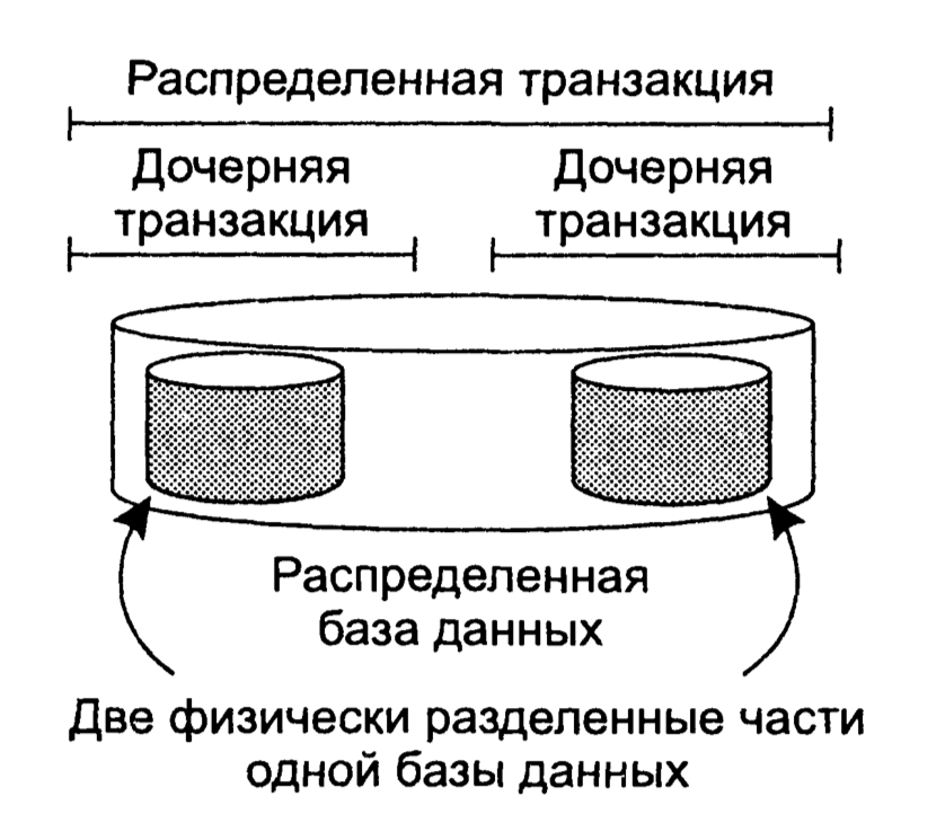
\includegraphics[width=0.8\textwidth]{assets/distributed/Transaction.png}
    \caption{Понятие распределенной транзакции}
\end{figure}

\subsubsection{Модель обработки транзакций}

Распределенная транзакция выполняет операции над данными, расположенными на нескольких сетевых узлах (серверах) одновременно. 
В распределенных СУБД обработка транзакций значительно усложняется, так как требуется обеспечить согласованность изменений на 
разных географически удаленных узлах базы данных, обеспечить атомарность и гарантировать целостность данных даже в случае сетевых 
сбоев или отказов отдельных серверов \autocite[гл. Введение]{Tanenbaum}.

Для обеспечения выполнения этих требований распределенные СУБД используют протоколы фиксации, которые будут описаны далее в разделе 
"Протоколы фиксации". Эти протоколы позволяет всем серверам, участвующим в транзакции, либо совместно подтвердить (зафиксировать), 
либо совместно отказаться (откатить) от ее выполнения. Такой подход позволяет сохранить принцип атомарности и согласованности транзакции 
вне зависимости от условий физического размещения данных и особенностей сетевой инфраструктуры.

Подробности об основных принципах обработки транзакций, журналирования, операциях фиксации и отката в контексте СУБД можно посмотреть 
в разделах «Механизмы обеспечения целостности СУБД» и "Механизмы, поддерживающие высокую готовность".

\subsubsection{Мониторы обработки транзакций}~\\

Мониторы обработки транзакций (Transaction Processing Monitor - TPM) — специализированное промежуточное программное обеспечение (middleware), 
обеспечивающее выполнение распределенных транзакций. TPM координируют работу нескольких серверов баз данных, гарантируя соблюдение ACID-свойств 
(атомарность, согласованность, изолированность, долговечность) для распределенных транзакций \autocite{TransactionMonitors}.

Архитектура приложений, использующих монитор обработки транзакций, состоит из трех частей \autocite{TPM}.

\begin{itemize}
    \item Уровень графического интерфейса - находится на компьютере клиента.
    \item Прикладной уровень - находится на множестве отдельных серверов приложений.
    \item Уровень данных - находится на отдельных серверах баз данных.
\end{itemize}

\begin{figure}[h!]
    \centering
    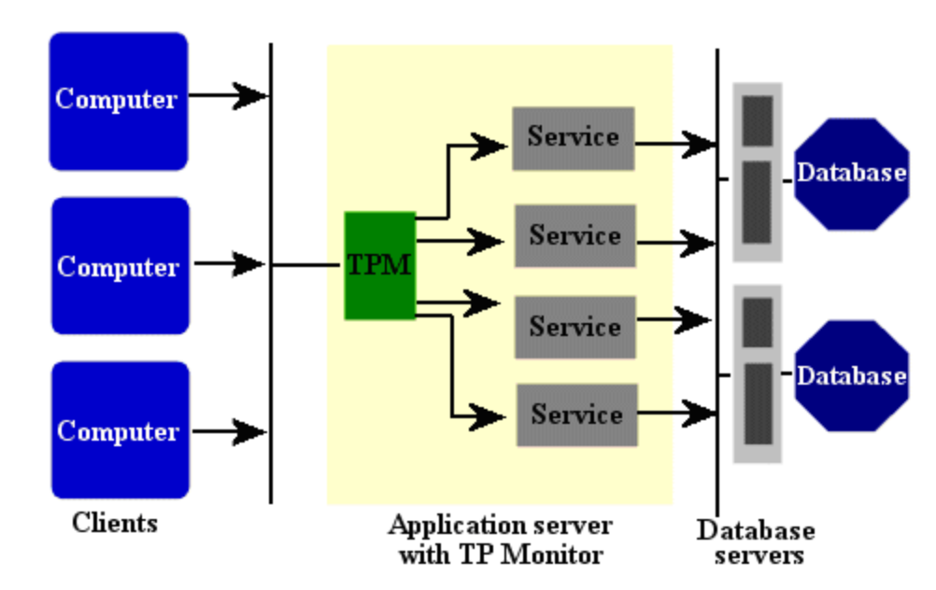
\includegraphics[width=0.8\textwidth]{assets/distributed/TPM.png}
    \caption{Архитектура приложений, использующих TPM}
\end{figure}

Архитектура системы обработки транзакций: 

\begin{itemize} 
    \item Прикладная программа — определяет границы транзакций, устанавливает конкретные действия, которые будет выполнять транзакция, и контролирует операции с данными, вызывая менеджеры ресурсов. 
    \item Менеджеры ресурсов — обеспечивают доступ к общим ресурсам, таким как базы данных, системы очередей сообщений и другие компоненты распределенной системы. 
    \item Менеджер транзакций — отвечает за создание транзакций, мониторинг их выполнения и координацию успешного завершения или отката при возникновении ошибок. 
\end{itemize}

Процесс обработки распределенной транзакции включает следующие шаги (рис. \ref{tpm_process}):

\begin{itemize}
    \item Клиент инициирует транзакцию, обращаясь к TPM, который генерирует идентификатор транзакции и создает контекст транзакции.
    \item Клиент взаимодействует с серверами ресурсов через удаленные вызовы процедур (RPC), передавая в каждом запросе контекст транзакции.
    \item Сервер извлекает контекст, регистрируется в TPM как участник транзакции и обрабатывает запрос.
    \item По завершении всех операций клиент уведомляет TPM о необходимости фиксации или отката транзакции.
    \item TPM координирует двухфазный протокол фиксации (2PC) между всеми участвующими серверами, обеспечивая атомарность транзакции \autocite{WebServices}.
(Рис. \ref{tpm_process}). 
\end{itemize}

\begin{figure}[h!]
    \centering
    \includegraphics[width=0.8\textwidth]{assets/distributed/TPM_arch.png}
    \caption{Процесс взаимодействия с TPM}
    \label{tpm_process}
\end{figure}

Примеры мониторов транзакций:
\begin{itemize}
  \item CICS (Система управления информацией о клиентах) для мэйнфреймов IBM;
  \item IBM Information Management System (IMS, точнее, её компонент IMS TM, также известный как IMS DC);
  \item ACMS (система управления приложениями) для OpenVMS;
  \item UNIVAC TIP;
  \item Transarc Encina;
  \item Oracle Tuxedo
\end{itemize}


\subsubsection{Корпоративная среда обработки транзакций}~\\

В этом разделе мы используем терминологию, предложенную автором статьи \autocite{TransactionMonitors}.

Корпоративная среда обработки транзакций  (Enterprise Transaction Processing — ETP) представляет собой комплексную инфраструктуру для выполнения распределенных транзакций в масштабах 
предприятия. Архитектура ETP строится на трех уровнях компьютерных систем \autocite{TransactionMonitors}:

\begin{itemize}
    \item Ряд 1: Персональные станции - рабочие станции пользователей, обеспечивающие интерфейс взаимодействия с системой;
    \item Ряд 2: Компьютеры под управлением ОС UNIX, на которых функционирует ядро TPM, и, как правило, реляционные СУБД, выступающие в качестве менеджера ресурсов;
    \item Ряд 3: Mainframe-системы или компьютеры под управлением UNIX c RISC-архитектурой процессоров;
\end{itemize}

Таким образом, среда обработки транзакций формируется из набора разнородных компьютеров (и соответствующих ОС),
ранжируемых от персональных компьютеров до мэйнфрейм-систем. TPM на базе UNIX представляет собой своего
рода "клей", который связывает вместе компьютеры трех рядов в открытую унифицированную среду обработки транзакций.

\begin{figure}[h!]
    \centering
    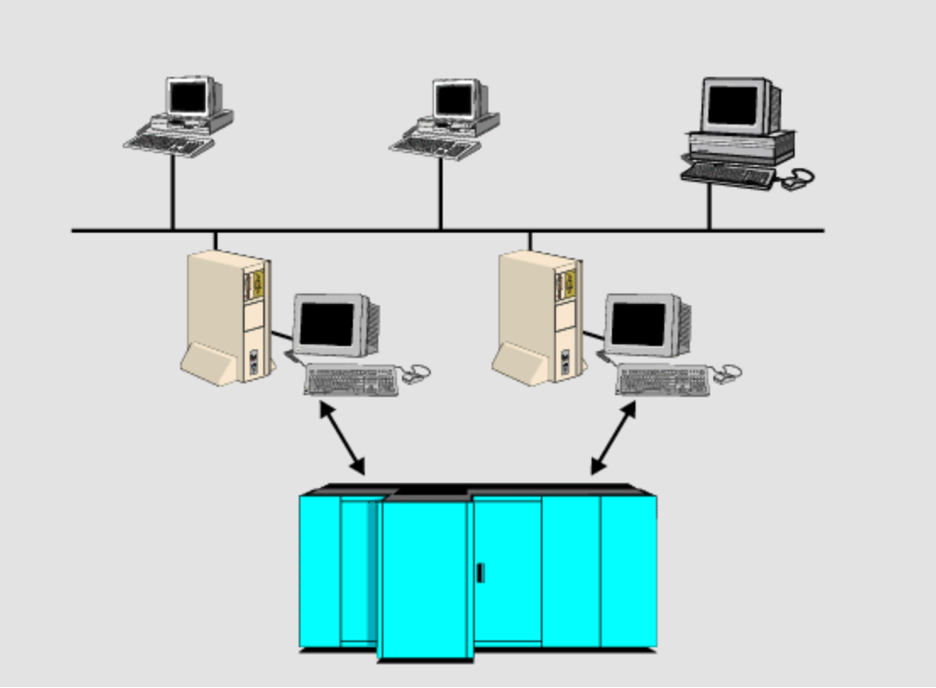
\includegraphics[width=0.8\textwidth]{assets/distributed/ETP.png}
    \caption{Промышленная среда обработки транзакций}
\end{figure}

При этом трехуровневая архитектура ETP характерна преимущественно для организаций, где исторически используются мэйнфреймы(типично для Европы 
и США). Для российских - более характерна двухуровневая архитектура ETP, включающая только клиентский уровень и серверы приложений/БД. При 
этом следует различать трехзвенную модель "клиент-сервер" (см. раздел 6.1 "Распределенные вычислительные среды"), относящуюся к логической 
организации, и архитектуру ETP, описывающую физическое распределение вычислительных ресурсов.

Ключом к интеграции систем, функционирующих на компьютерах различных рядов, является специализированный
интерфейс прикладного программирования ATMI (Application Transaction Manager Interface), обеспечивающий \autocite{TransactionMonitors}:
\begin{itemize}
    \item для ряда 1 - формирование и передачу запросов от клиентов к серверам, выполняющимся на компьютерах ряда 2
    \item для ряда 2 - обработку запросов, поступающих от компьютера ряда 1 (в том числе и с
    обращением к менеджеру ресурсов), и, по необходимости, формирование и направление
    запросов к серверам, выполняющимся на компьютерах ряда 3
    \item для ряда 3 - обработку запросов, поступающих от серверов ряда 2
\end{itemize}

\subsection{Протоколы фиксации}

Протоколы фиксации транзакций представляют собой механизм, обеспечивающий атомарность 
выполнения транзакций в распределенных базах данных. Их основная задача — гарантировать, что все участвующие в 
транзакции узлы либо зафиксируют изменения, либо откатят их, даже при возникновении сетевых сбоев или отказе отдельных 
компонентов системы. \autocite{FixProtocols}

Распределенная транзакция имеет дело с разделяемыми данными на нескольких географически рассредоточенных серверах. 
На заключительном этапе каждый сервер должен выполнить некоторое количество завершающих операций, предписанных транзакцией. 
На этой стадии все серверы, невзирая на отказы, должны согласовать окончательное решение — транзакция должна быть фиксирована 
или прервана. Даже одного голоса, поданного за прерывание транзакции, достаточно для того, чтобы транзакция была прервана.
 Какое бы решение ни было принято, оно должно быть передано всем участникам транзакции. 
 
Условия задачи атомарного завершения (commitment):

\begin{itemize}
    \item Согласие (Agreement). Все процессы принимают одно и то же решение.
    \item Валидность (Validity). Если один из процессов голосует за прерывание, тогда транзакция должна быть прервана. 
    Если все процессы голосуют за фиксацию, и отказы отсутствуют, тогда транзакция должна быть фиксирована.
    \item Завершение (Termination). Все корректно работающие процессы должны в конечном счете прийти к финальному 
    решению.
\end{itemize}

Протоколы фиксации спроектированы так, чтобы работать в асинхронной системе, в которой серверы могут отказывать и сообщения 
могут теряться. Свойство согласия подразумевает, что все серверы достигают одного и того же решения \autocite{Fix}.

\subsubsection{Распределенная однофазная фиксация}

Распределенная однофазная фиксация (Distributed One-Phase Commit, 1PC) представляет собой упрощенный протокол 
атомарной фиксации транзакций в распределенных базах данных, требующий всего одного раунда обмена сообщениями 
между координатором и участниками.

Начиная транзакцию, клиентское приложение делает запрос одному из процессов службы поддержки транзакций на ближайшем 
доступном сервере. Этот процесс становится координатором транзакции. Другие серверы, вовлеченные в эту транзакцию,
называются участниками транзакции.

Координатор распределяет работу по осуществлению транзакции между участниками и на заключительном этапе посылает 
сообщение фиксация (COMMIT) или прерывание (ABORT) всем участникам транзакции и ждет, пока все они пришлют подтверждения 
о том, что распоряжение выполнено. Это так называемая однофазная фиксация. При этом не исключено, что вследствие локальных 
проблем (подобных отказу компонентов или конфликтам параллельного исполнения) некоторые участники не смогут проинформировать
 о своем решении координатора и других участников. Поскольку решение должно быть принято в течение одной фазы, координатор и 
 корректные участники, не будучи оповещенными о проблемах других участников, не смогут прийти к согласию относительно возможности
фиксации или прерывания транзакции. Для практического применения необходима более сложная схема \autocite{Fix}.

\subsubsection{Распределенная двухфазная фиксация}

Протокол двухфазной фиксации (Two-phase Commit Protocol, 2РС) был спроектирован, чтобы преодолеть ограничения протокола
однофазной фиксации. В течение первой фазы координатор посылает сообщение VOTE каждому участнику, спрашивая у них, намерены 
ли они фиксировать транзакцию или прерывать ее. Далее координатор анализирует собранные ответы.

Если все серверы готовы фиксировать транзакцию, тогда в течение второй фазы координатор посылает всем участникам сообщение COMMIT. 
В противном случае, если по крайней мере один из участников проголосовал за прерывание, координатор посылает всем участникам сообщение ABORT.

Каждый участник после посылки своего голоса ждет получения сообщения (COMMIT или ABORT) от координатора. После получения сообщения каждый 
участник локально выполняет необходимые действия по фиксации или прерыванию транзакции. Очевидно, что условия согласия, валидности и 
завершения выполняются, и следовательно, протокол двухфазного подтверждения решает задачу распределенной фиксации транзакции \autocite{Fix}.

\textbf{Обработка ошибок}

Протокол 2РС может попасть в трудную ситуацию в случае сбоя. Например, один из участников может отказать из-за поломки и, следовательно, не ответить. 
Сообщения также могут быть потеряны. Это делает реализацию протокола двухфазной фиксации нетривиальной. В варианте чисто асинхронного исполнения, 
когда координатор или участник блокируются в ожидании сообщения, они не смогут узнать, что произошло: поломка сервера, потеря или задержка сообщения. 

На практике для обнаружения потерь и отказов процессов часто используют таймауты, но это не считается надежным решением. Поэтому в случае любого сомнения 
систему принято возвращать к безопасной конфигурации путем прерывания всех транзакций. Некоторые варианты отказов и способы борьбы с ними суммированы ниже.

Вариант 1. Если (на фазе 1) координатор не получает ответа по крайней мере от одного участника в период таймаута, тогда он решает прервать транзакцию и 
рассылает всем участникам сообщение ABORT.

Вариант 2. Если (на фазе 1) участник не получает сообщения VOTE от координатора в течение определенного таймаута, предполагая, что координатор отказал или 
сообщение VOTE потеряно или задержано, он посылает сообщение ABORT координатору и затем локально прерывает транзакцию.

Вариант 3. Если (на фазе 2) участник не получает сообщение COMMIT или ABORT от координатора в течение оговоренного периода времени (это может быть случай 
поломки координатора после посылки сообщений ABORT или COMMIT только части серверов), тогда он остается в состоянии неопределенности до тех пор, пока 
координатор не восстановится и не реинсталлируется в системе. При этом на неопределенный период ресурсы могут оставаться заблокированными, мешая другим 
транзакциям. По этой причине протокол 2РС также называют протоколом блокирующего подтверждения. Блокировка ресурсов — один из недостатков протокола 
двухфазной фиксации \autocite{Fix}.

\subsubsection{Распределенная трехфазная фиксация}

Протокол трёхфазной фиксации (3PC) — это расширение протокола двухфазной фиксации (2PC), которое позволяет избежать проблемы блокировки при определённых условиях. В частности, 
предполагается, что не происходит разделения сети на части и не более k узлов выходят из строя, где «k» — заранее заданное число. При соблюдении упомянутых условий протокол позволяет 
избежать блокировки за счёт введения дополнительной третьей фазы, в которой в принятии решения о фиксации участвуют несколько узлов.

Вместо того чтобы напрямую сохранять решение о фиксации в постоянном хранилище, координатор сначала гарантирует, что по крайней мере «k» других узлов знают, что он намерен зафиксировать 
транзакцию.

В ситуации, когда координатор выходит из строя, оставшиеся узлы должны сначала выбрать нового координатора. Этот новый координатор проверяет состояние протокола на оставшихся узлах. 
Если координатор решил зафиксировать транзакцию, то по крайней мере один из других «k» узлов, о которых он сообщил, будет работать и обеспечит соблюдение решения о фиксации транзакции. 
Новый координатор перезапускает третью фазу протокола, если какой-либо из оставшихся узлов знал, что старый координатор намеревался зафиксировать транзакцию. В противном случае новый 
координатор прерывает транзакцию.

При опросе участников, если он обнаруживает, что некоторые узлы находятся на этапе фиксации, он предполагает, что предыдущий координатор перед сбоем принял решение о фиксации.
Следовательно, он может завершить протокол фиксацией. Аналогичным образом, если участник отвечает, что он не получил команду на подготовку к фиксации, то новый координатор может 
предположить, что предыдущий координатор потерпел неудачу ещё до того, как начал подготовку к фиксации. Следовательно, он может с уверенностью предположить, что ни один другой участник 
не зафиксировал изменения, и поэтому он может безопасно прервать транзакцию \autocite{3PC}.

Разницу между трёхфазным и двухфазным протоколами фиксации можно понять по рисункам \ref{2pc} и \ref{3pc}.

\begin{figure}[h!]
    \centering
    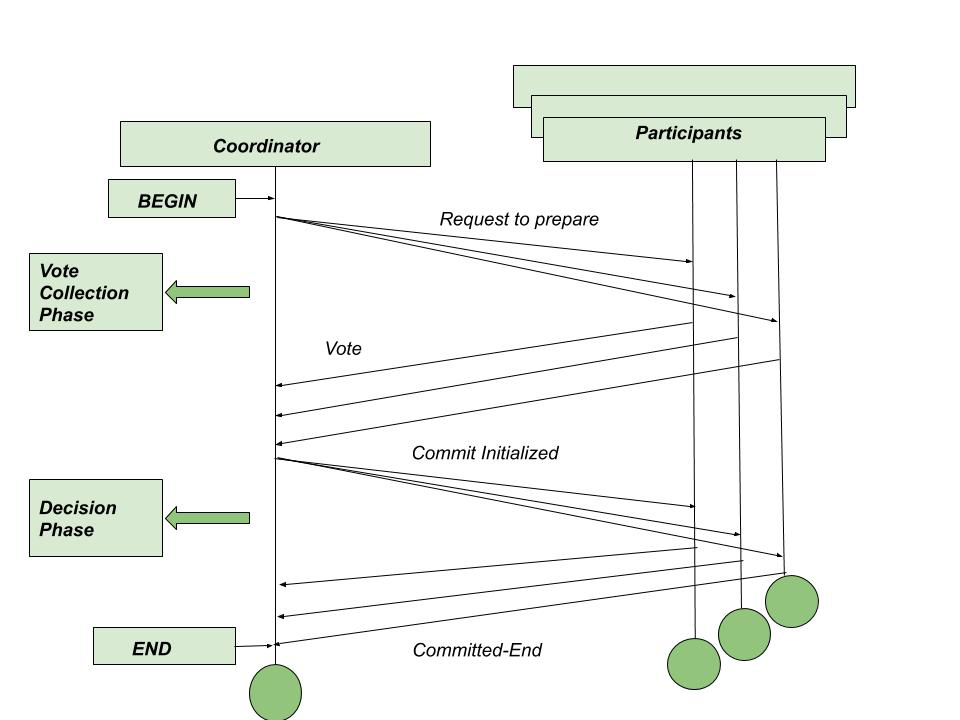
\includegraphics[width=0.8\textwidth]{assets/distributed/2PhaseCommit.png}
    \caption{Протокол двухфазной фиксации}
    \label{2pc}
\end{figure}

\begin{figure}[h!]
    \centering
    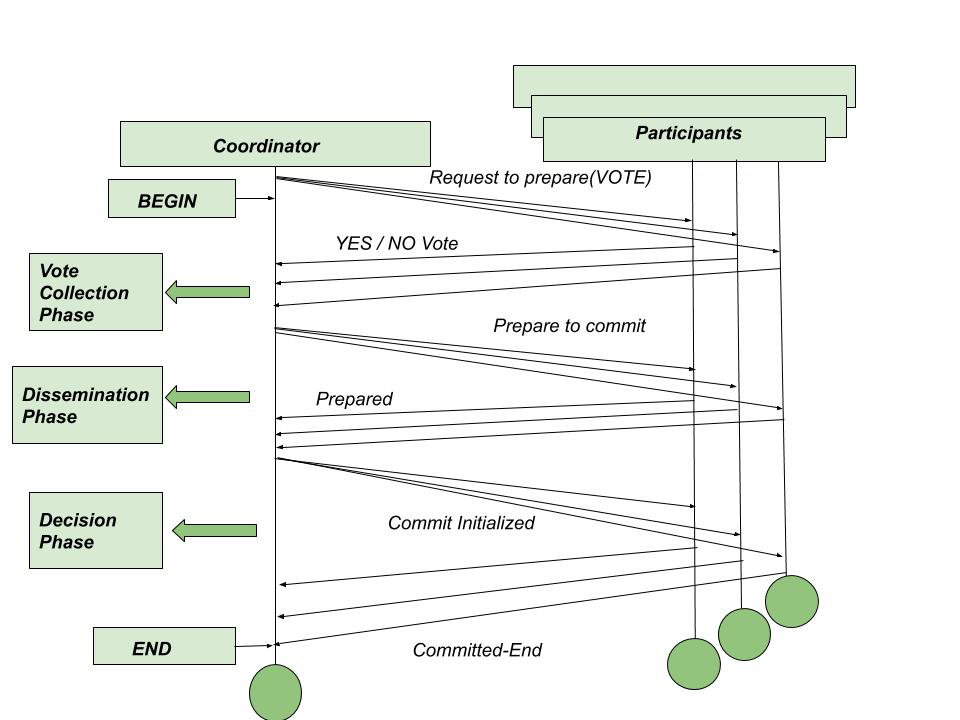
\includegraphics[width=0.8\textwidth]{assets/distributed/3PhaseCommit.png}
    \caption{Протокол трехфазной фиксации}
    \label{3pc}
\end{figure}

Таким образом, между фазами запроса на фиксацию и окончательной фиксацией в отличие от 2PC добавляется фаза предварительной фиксации:

\begin{itemize}
    \item Координатор отправляет всем участникам сообщение \texttt{prepare to commit}
    \item Участники выполняют все необходимые операции для подготовки к окончательной фиксации
    \item Участники переходят в состояние "готов к фиксации"
    \item Каждый участник отправляет координатору подтверждение о готовности (\texttt{ACK})
\end{itemize}

\subsubsection{Защищенные протоколы фиксации}

Некоторые примеры с ссылками на описание протоколов:

\begin{itemize}
    \item BFT-2PC \autocite{BFT-2PC}
    \item PBFT \autocite{PBFT}
    \item PoW (Proof of Work Commit) \autocite{PoS_PoW}
    \item PoS (Proof of Stake Commit) \autocite{PoS_PoW}
\end{itemize}

\paragraph{Обработка распределенных транзакций в базах данных с многоуровневой секретностью (MLS)}~\\

Для внедрения разграничения доступа в системы  управления  базами  данных  (СУБД  -
DBMS)  предложены некоторые решения. Однако эти решения не достаточно
эффективны, поэтому рассмотрим понятие  системы
управления  базами  данных  с  многоуровневым  разграничением доступа (MLS/DBMS).

Известно, что в MLS/DBMS не ко всем данным, содержащимся в  базе
данных, доступ осуществляется одинаково. Однако современные СУБД, как
правило,  не имеют адекватных средств диагностики и механизма определения
того, что пользователь имеет возможность доступа только  к  тем
данным,  которые являются релевантными. Таким образом, MLS/DBMS отличается
от соответствующих DBMS,  по крайней  мере,  следующими  двумя
особенностями \autocite{SecureFix}:
\begin{itemize}
    \item каждый элемент данных в базе данных связан с уровнем доступа
    \item доступ пользователя к данным должен контролироваться релевантностью для данного пользователя
\end{itemize}
Разработка сервиса MLS/DBMS в современных компьютерных  системах
представляет  много  проблем. До настоящего времени внедрение многоуровневого
разграничения доступа в операционную  систему  представляет
собой  значительные трудности. Решение этой проблемы в виде аббревиатуры
обозначается ТСВ. Хотя в разрешении вопросов ТСВ  для  удаленных
пользователей  в  MLS/DBMS вводятся компромиссы, остается много проблем,
которые требуется разрешать. Наиболее очевидная проблема состоит
в том, что вопросы классификации в СУБД значительно  сложнее,  чем  в
файловых  системах  и могут быть сложнее реализованы. Другая проблема
состоит в том, что для классификации данных,  содержащих  контекстные
представления,  временные параметры, их композицию, необходимы унифицированные базы данных 

Подробнее можно почитать в \autocite{SecureFix}.

\subsubsection{Алгоритмы консенсуса}

\paragraph{Проблема консенсуса в распределённых системах}~\\ 

\textbf{Проблема консенсуса} — фундаментальная задача распределённых систем, требующая согласования общего решения между узлами в условиях возможных сбоев, задержек сообщений или 
неисправностей участников. Формально, каждый узел системы предлагает своё начальное значение, и все корректные узлы должны прийти к единому решению, удовлетворяющему следующим условиям \autocite{Consensus}: 

\begin{itemize} 
    \item \textbf{Согласованность (Agreement)}: Все узлы принимают одно и то же значение. 
    \item \textbf{Целостность (Integrity)}: Решение должно быть предложено хотя бы одним узлом. 
    \item \textbf{Завершаемость (Termination)}: Каждый корректный узел в конечном итоге принимает решение. 
\end{itemize}

\paragraph{Теоретические ограничения}~\\ 

В распределённых системах достижение консенсуса осложнено теоретическими ограничениями: 

\begin{itemize} 
    \item \textbf{Теорема FLP} (Fischer, Lynch, Paterson, 1985): В асинхронной системе с хотя бы одним отказом узла консенсус невозможен, если возможна произвольная задержка сообщений \autocite{Fischer1985}. 
    \item \textbf{CAP-теорема} (Brewer, 2000): Система может гарантировать только два из трёх свойств: согласованность (Consistency), доступность (Availability), устойчивость к разделению (Partition tolerance) \autocite{Brewer2012}. 
\end{itemize}

\paragraph{Типы отказов}~\\ 

Алгоритмы консенсуса классифицируются по типу отказов, которые они могут преодолеть: 

\begin{itemize} 
    \item \textbf{Аварийные отказы (Crash faults)}: Узел перестаёт отвечать, но не действует злонамеренно. 
    \item \textbf{Византийские отказы (Byzantine faults)}: Узел может произвольно искажать данные или нарушать протокол \autocite{Castro1999}. 
\end{itemize}

\paragraph{Примеры алгоритмов консенсуса}~\\ 

\begin{itemize} 
    \item \textbf{Paxos}: суть алгоритма заключается в процессе, в ходе которого участники системы (proposers, acceptors и learners) взаимодействуют по строго определенным правилам, 
    чтобы прийти к единому согласованному решению. Основные этапы алгоритма включают предложение значения (proposal), голосование за предложение и подтверждение(acceptance) предложенного 
    значения большинством узлов \autocite{paxos}. 
    \item \textbf{Raft}: для обеспечения консенсуса среди серверов выбирается лидер, который принимает запросы на изменение данных и координирует их распространение на остальные узлы. 
    При отказе лидера автоматически проводится новый выбор лидера, что обеспечивает устойчивость и согласованность системы. \autocite{raft}. 
\end{itemize}


\subsection{Тиражирование данных}

\textbf{Тиражирование данных} - это асинхронный перенос изменений объектов исходной базы данных (source database)
в базы данных, принадлежащие к различным узлам распределенной системы. Тиражирование данных может происходит
двумя различными способами: \textbf{шардингом} (или, иначе говоря, шардированием, фрагментацией) и \textbf{репликацией}.

\subsubsection{Шардинг (sharding)}

\textbf{Шардинг} — это метод проектирования базы данных, при котором данные разделяются на группы и хранятся на разных серверах. Это улучшает производительность, поскольку данные хранятся там, где они чаще всего используются, что уменьшает сетевой трафик.

Существуют два основных вида шардирования: \textbf{горизонтальное} и \textbf{вертикальное}. Они соответствуют операциям сокращения и проекции в реляционных базах данных. Важно, чтобы все фрагменты были независимыми, то есть ни один из фрагментов не может быть представлен как производный от других фрагментов.

Одной из ключевых особенностей шардинга является поддержка независимости от шардирования. Это означает, что пользователи могут работать так, как если бы данные в действительности были вовсе не шардированы. Это упрощает разработку пользовательских программ и выполнение терминальных операций.

Если обеспечивается независимость от шардирования, пользователи получают данные в виде представления, в котором шарды логически скомбинированы с помощью операций соединения и объединения. Задачей системного оптимизатора является определение шардов, к которым требуется доступ для выполнения запросов пользователя.
\autocite{IntroBD2014}

\paragraph{Алгоритмы шардинга} ~\\
Ранее уже упоминалось о двух основных вида шардинга: \textit{горизонтальный} и \textit{вертикальный}. Стоит их разобрать по подробнее и
рассказать и про другие виды шардирования, такие как шардинг на основе каталогов и шардинг на основе ключей.

\paragraph{Горизонтальное шардирование} ~\\
В этом методе мы разбиваем данные на основе диапазонов заданного значения, присущего каждой сущности. Допустим, у вас
есть база данных имен ваших онлайн-клиентов и информации об электронной почте. Вы можете разделить эту информацию на
два осколка. В одном осколке вы можете хранить информацию о клиентах, чье имя начинается с A-P, а в другом - информацию
об остальных клиентах.

\begin{figure}[H]
    \centering
    \includegraphics[width=100mm]{assets/distributed/Horizontal-Sharding}
    \caption{Горизонтальное шардирование}
    \label{fig:Horizontal-Sharding}
\end{figure}

\textbf{Горизонтальное шардирование} - самый простой метод сегментирования для реализации. Каждый осколок содержит
другой набор данных, но все они имеют ту же схему, что и исходная база данных. В этом методе вам просто нужно
определить, в какой диапазон попадают ваши данные, а затем вы можете сохранить запись в соответствующий шард. Этот
метод лучше всего подходит для хранения нестатических данных (например, хранение контактной информации студентов
колледжа).

Недостатком этого метода является то, что данные могут быть неравномерно распределены по шардам. В приведенном выше
примере у вас может быть много клиентов, имена которых попадают в категорию A-P. В таких случаях первый осколок должен
будет взять на себя больше нагрузки, чем второй, и это может стать узким местом системы. \autocite{DatabaseSharding}

\paragraph{Вертикальное шардирование} ~\\
В этом методе мы разделяем весь столбец из таблицы и помещаем эти столбцы в новые отдельные таблицы. Данные полностью
независимы от одного раздела к другому. Кроме того, каждый раздел содержит как отдельные строки, так и столбцы. Возьмем,
к примеру, функции Twitter. Мы можем разделить различные функции объекта на разные сегменты на разных машинах. В
Твиттере у пользователя может быть профиль, количество подписчиков и некоторые твиты, опубликованные им самим. Мы можем
разместить профили пользователей на одном осколке, подписчиков - на втором, а твиты - на третьем.

\begin{figure}[H]
    \centering
    \includegraphics[width=100mm]{assets/distributed/Vertical-Sharding}
    \caption{Вертикальное шардирование}
    \label{fig:Vertical-Sharding}
\end{figure}

В этом методе вы можете отделить и обработать критическую часть (например, профили пользователей) от некритической части
ваших данных (например, сообщения в блоге) по отдельности и построить вокруг нее различные модели репликации и
согласованности. Это одно из главных преимуществ этого метода.

Основным недостатком этой схемы является то, что для ответа на некоторые запросы вам, возможно, придется комбинировать
данные из разных шардов, что неоправданно увеличивает сложность разработки и эксплуатации системы. Кроме того, если
ваше приложение будет расти позже, и вы добавите в него еще несколько функций, вам придется дополнительно сегментировать
базу данных с конкретными функциями на нескольких серверах. \autocite{DatabaseSharding}

\paragraph{Шардинг на основе каталогов} ~\\
В этом методе мы создаем и поддерживаем службу поиска или таблицу поиска для исходной базы данных. В основном мы
используем ключ осколка для таблицы поиска и делаем сопоставление для каждого объекта, существующего в базе данных.
Таким образом, мы отслеживаем, какие осколки базы данных содержат какие данные.

Таблица поиска содержит статический набор информации о том, где можно найти конкретные данные. На приведенном выше
изображении вы можете видеть, что мы использовали зону доставки в качестве ключа осколка. Во-первых, клиентское
приложение запрашивает службу поиска, чтобы узнать осколок (раздел базы данных), на котором размещены данные. Когда
служба поиска возвращает осколок, она запрашивает/обновляет этот осколок.

\begin{figure}[H]
    \centering
    \includegraphics[width=100mm]{assets/distributed/Directory-Based-Sharding}
    \caption{Шардинг на основе каталогов}
    \label{fig:Directory-Based-Sharding}
\end{figure}

Сегментация на основе каталогов гораздо более гибкая, чем сегментация на основе диапазонов и ключей. В сегменте на
основе диапазонов вы обязаны указать диапазоны значений. В key-based вы обязаны использовать фиксированную хэш-функцию,
которую трудно изменить позже. При таком подходе вы можете использовать любой алгоритм, который хотите назначить для
записей данных в сегменты. Кроме того, при таком подходе легко динамически добавлять шарды.

Основным недостатком этого подхода является единственная точка отказа таблицы поиска. Если он будет поврежден или не
удался, это повлияет на запись новых данных или доступ к существующим данным из таблицы. \autocite{DatabaseSharding}

\paragraph{Шардинг на основе ключей} ~\\
Этот метод также известен как сегментация на основе хэша. Здесь мы берем значение объекта, такого как идентификатор
клиента, адрес электронной почты клиента, IP-адрес клиента, почтовый индекс и т. д., и мы используем это значение в
качестве входных данных хэш-функции. Этот процесс генерирует хэш-значение, которое используется для определения того,
какой шард нам нужно использовать для хранения данных. Мы должны иметь в виду, что значения, введенные в хэш-функцию,
должны поступать из одного и того же столбца (ключ осколка), чтобы данные размещались в правильном порядке и
согласованно. В принципе, ключи осколков действуют как первичный ключ или уникальный идентификатор для отдельных строк.

\begin{figure}[H]
    \centering
    \includegraphics[width=100mm]{assets/distributed/Keybased-Sharding}
    \caption{Шардинг на основе ключей}
    \label{fig:Keybased-Sharding}
\end{figure}

Рассмотрим пример, что у вас есть 3 сервера баз данных, и каждый запрос имеет идентификатор приложения, который
увеличивается на 1 каждый раз, когда регистрируется новое приложение. Чтобы определить, на каком сервере должны быть
размещены данные, мы выполняем операцию по модулю для этих приложений id с номером 3. Затем остаток используется для
идентификации сервера для хранения наших данных.

Недостатком этого метода является эластичная балансировка нагрузки, что означает, если вы попытаетесь динамически
добавлять или удалять серверы баз данных, это будет сложный и дорогостоящий процесс. Например, в приведенном выше
примере, если вы добавите еще 5 серверов, вам нужно добавить больше соответствующих хэш-значений для дополнительных
записей. Кроме того, большинство существующих ключей необходимо переназначить на их новое, правильное хэш-значение,
а затем перенести на новый сервер. Хэш-функция должна быть изменена с модуля 3 на модуль 8. В то время как миграция
данных действует, как новые, так и старые хэш-функции не будут действительны. Во время миграции ваше приложение не
сможет обслуживать большое количество запросов, и вы будете испытывать простои для своего приложения до завершения
миграции. \autocite{DatabaseSharding}

\paragraph{Географический шардинг} ~\\
Шардирование по географическому признаку позволяет хранить определенные данные вблизи своих потребителей и
удовлетворять нормативным требованиям, когда данные должны находиться в определенной юрисдикции. Однако данный способ
шардирования не является самодостаточным: шарды могут быть загружены не равномерно, и отличие может быть на порядки.
На пример, экземпляр базы данных, хранящий данные пользователей Москвы и Московской области, будет намного превышать
другой экземпляр базы данных, который хранит информацию о пользователях из Владимира. Таким образом, недостатком
данного метода является необходимость дополнительного использования других методов шардирования.

\subsubsection{Репликация} ~\\

\textbf{Репликация} — это процесс изменения одного набора данных, называемого репликой, в ответ на изменения другого
набора данных, называемого основным. Репликация желательна по крайней мере по двум причинам. Во-первых, она способна
обеспечить более высокую производительность, поскольку приложения смогут обрабатывать локальные копии вместо того,
чтобы устанавливать связь с удаленными узлами. Во-вторых, наличие репликации может также обеспечивать более высокую
степень доступности, поскольку любой реплицируемый объект остается доступным для обработки (по крайней мере, для выборки
данных), пока хотя бы одна реплика в системе остается доступной. Главным недостатком репликации, безусловно, является
то, что если реплицируемый объект обновляется, то и все его копии должны быть обновлены (проблема распространения
обновлений).

Очевидно, что репликация, как и шардирование, теоретически должна быть "прозрачной для пользователя". Другими словами,
система, которая поддерживает репликацию данных, должна также поддерживать независимость от репликации (иногда говорят
"прозрачность репликации"). Для пользователей должна быть создана такая среда, чтобы они, по крайней мере, с логической
точки зрения могли считать, что в действительности данные не дублируются. Независимость от репликации (как и
независимость от шардирования) является весьма желательной, поскольку она упрощает создание пользовательских программ и
выполнение терминальных операций. В частности, независимость от репликации позволяет создавать и уничтожать дубликаты в
любой момент в соответствии с изменяющимися требованиями, не затрагивая при этом никакие из пользовательских программ
или терминальных операций.

Из требования независимости от репликации следует, что к обязанностям системного оптимизатора также относится
определение, какой именно из физических дубликатов будет применен для доступа к данным при выполнении каждого
введенного пользователем запроса. \autocite{IntroBD2014}

Можно выделить три \textbf{подхода к репликации}:
\begin{itemize}
    \item Блочная репликация на уровне системы хранения данных;
    \item Физическая репликация на уровне СУБД;
    \item Логическая репликация на уровне СУБД.
\end{itemize}

\paragraph{Блочная репликация} ~\\
При блочной репликации каждая операция записи выполняется не только на основном диске, но и на резервном. Таким образом
тому на одном массиве соответствует зеркальный том на другом массиве, с точностью до байта повторяющий основной том.

К достоинствам такой репликации можно отнести простоту настройки и надёжность. Записывать данные на удалённый диск может
либо дисковый массив, либо нечто (устройство или программное обеспечение), стоящее между хостом и диском. Если дисковый
массив не способен реплицировать данные, между хостом и массивом может быть установлен агент, осуществляющей запись на
два массива сразу. Агент может быть как отдельным устройством, так и программным компонентом. В отличие от дискового
массива, который может работать только с таким же массивом или, как минимум, с массивом того же производителя, агент
может работать с совершенно разными дисковыми устройствами.

Главное назначение блочной репликации – обеспечение отказоустойчивости. Если база данных потеряна, то можно
перезапустить её с использованием зеркального тома. Блочная репликация хороша своей универсальностью, но за
универсальность приходится платить.

Во-первых, никакой сервер не может работать с зеркальным томом, поскольку его операционная система не может управлять
записью на него; с точки зрения наблюдателя данные на зеркальном томе появляются сами собой. В случае аварии (отказ
основного сервера или всего ЦОДа, где находится основной сервер) следует остановить репликацию, размонтировать основной
том и смонтировать зеркальный том. Как только появится возможность, следует перезапустить репликацию в обратном
направлении.

Во-вторых, сама СУБД на резервном сервере может быть запущена только после монтирования диска. В некоторых операционных
системах, например, в Solaris, память под кеш при выделении размечается, и время разметки пропорционально объёму
выделяемой памяти, то есть старт экземпляра будет отнюдь не мгновенным. Плюс ко всему кеш после рестарта будет пуст.

В-третьих, после запуска на резервном сервере СУБД обнаружит, что данные на диске неконсистентны, и нужно потратить
значительное время на восстановление с применением журналов повторного выполнения: сначала повторить те транзакции,
результаты которых сохранились в журнале, но не успели сохраниться в файлы данных, а потом откатить транзакции, которые
к моменту сбоя не успели завершиться. \autocite{Replication}

\paragraph{Физическая репликация (master-slave)} ~\\
Журналы (redo log или write-ahead log) содержат все изменения, которые вносятся в файлы базы данных. Идея физической
репликации состоит в том, что изменения из журналов повторно выполняются в другой базе (реплике), и таким образом данные
в реплике повторяют данные в основной базе байт-в-байт \autocite{PhysLogPeplic}.

Журналы СУБД не предназначены для использования вне этой платформы, их формат не документируется и может меняться без
предупреждения. Отсюда совершенно естественное требование, что физическая репликация возможна только между экземплярами
одной и той же версии одной той же СУБД. Отсюда же возможные ограничения на операционную систему и архитектуру
процессора, которые тоже могут влиять на формат журнала.

Естественно, никаких ограничений на модели СХД физическая репликация не накладывает. Более того, файлы в базе-реплике
могут располагаться совсем по-другому, чем на базе-источнике – надо лишь описать соответствие между томами, на которых
лежат эти файлы.

Запись данных в реплику невозможна, поскольку изменения в неё приходят побайтно, и реплика не может обеспечить
конкурентное исполнение своих запросов. В случае повреждения файла в основной базе можно просто скопировать
соответствующий файл с реплики. Однако стоит учесть, что файл на реплике может быть не идентичен файлу в основной базе:
когда файл расширяется, новые блоки в целях ускорения ничем не заполняются, и их содержимое случайно. База может
использовать не всё пространство блока (например, в блоке может оставаться свободное место), но содержимое
использованного пространства совпадает с точностью до байта \autocite{PhysLogPeplic}.

Физическая репликация может быть как синхронной, так и асинхронной. При асинхронной репликации всегда есть некий набор
транзакций, которые завершены на основной базе, но ещё не дошли до резервной, и в случае перехода на резервную базу при
сбое основной эти транзакции будут потеряны. При синхронной репликации завершение операции commit означает, что все
журнальные записи, относящиеся к данной транзакции, переданы на реплику. Важно понимать, что получение репликой журнала
не означает применения изменений к данным. При потере основной базы транзакции не будут потеряны, но если приложение
пишет данные в основную базу и считывает их из реплики, то у него есть шанс получить старую версию этих данных \autocite{PhysLogPeplic}.

Физическая репликация базы данных имеет множество преимуществ перед репликацией средствами СХД \autocite{PhysLogPeplic}:
\begin{itemize}
    \item объём передаваемых данных меньше за счёт того, что передаются только журналы, но не файлы с данными; эксперименты показывают уменьшение трафика в 5-7 раз;
    \item переключение на резервную базу происходит значительно быстрее: экземпляр-реплика уже поднят, поэтому при переключении ему нужно лишь откатить активные транзакции; более того, к моменту сбоя кеш реплики уже прогрет;
    \item на реплике можно выполнять запросы, сняв тем самым часть нагрузки с основной базы. В частности, реплику можно использовать для создания резервных копий.
\end{itemize}

\paragraph{Логическая репликация (active-active)} ~\\
Все изменения в базе данных происходят в результате вызовов её API – например, в результате выполнения SQL-запросов.
Очень заманчивой кажется идея выполнять одну и ту же последовательность запросов на двух разных базах. Для репликации
необходимо придерживаться двух правил \autocite{PhysLogPeplic}:
\begin{itemize}
    \item нельзя начинать транзакцию, пока не завершены все транзакции, которые должны закончиться раньше; Так на рисунке ниже нельзя запускать транзакцию D, пока не завершены транзакции A и B;
    \item нельзя завершать транзакцию, пока не начаты все транзакции, которые должны закончиться до завершения текущей транзакции; Так на рисунке ниже даже если транзакция B выполнилась мгновенно, завершить её можно только после того, как начнётся транзакция C.
\end{itemize}

\begin{figure}[H]
    \centering
    \includegraphics[width=100mm]{assets/distributed/ReplicationExample}
    \caption{Пример репликации}
    \label{fig:ReplicationExample}
\end{figure}

\textbf{Репликация команд (statement-based replication)} реализована, например, в MySQL. К сожалению, эта простая схема не
приводит к появлению идентичных наборов данных – тому есть две причины \autocite{PhysLogPeplic}.
\begin{itemize}
    \item не все API детерминированы. Например, если в SQL-запросе встречается функция now() или sysdate(), возвращающая текущее время, то на разных серверах она вернёт разный результат – из-за того, что запросы выполняются не одновременно. Кроме того, к различиям могут привести разные состояния триггеров и хранимых функций, разные национальные настройки, влияющие на порядок сортировки, и многое другое.
    \item репликацию, основанную на параллельном исполнении команд, невозможно корректно приостановить и перезапустить. На рисунке выше если репликация остановлена в момент T1 транзакция B должна быть прервана и откачена. При перезапуске репликации исполнение транзакции B может привести реплику к состоянию, отличному от состояния базы-источника: на источнике транзакция B началась до того, как закончилась транзакция A, а значит, она не видела изменений, сделанных транзакцией A. Репликация запросов может быть остановлена и перезапущена только в момент T2, когда в базе нет ни одной активной транзакции. Разумеется, на сколько-нибудь нагруженной промышленной базе таких моментов не бывает.
\end{itemize}

Обычно для логической репликации используют детерминированные запросы. Детерминированность запроса обеспечивается двумя
свойствами:
\begin{itemize}
    \item запрос обновляет (или вставляет, или удаляет) единственную запись, идентифицируя её по первичному (или уникальному) ключу;
    \item все параметры запроса явно заданы в самом запросе.
\end{itemize}

В отличие от \textbf{репликации команд (statement-based replication)} такой подход называется \textbf{репликацией
записей (row-based replication)} \autocite{PhysLogPeplic}.

База-реплика открыта и доступна не только на чтение, но и на запись. Это позволяет использовать реплику для выполнения
части запросов, в том числе для построения отчётов, требующих создания дополнительных таблиц или индексов. Важно
понимать, что логическая реплика будет эквивалентна исходной базе только в том случае, если в неё не вносится никаких
дополнительных изменений

Логическая репликация предоставляет ряд возможностей, отсутствующих в других видах репликации \autocite{PhysLogPeplic}:
\begin{itemize}
    \item настройка набора реплицируемых данных на уровне таблиц (при физической репликации – на уровне файлов и табличных пространств, при блочной репликации – на уровне томов);
    \item построение сложных топологий репликации – например, консолидация нескольких баз в одной или двунаправленная репликация;
    \item уменьшение объёма передаваемых данных;
    \item репликация между разными версиями СУБД или даже между СУБД разных производителей;
    \item обработка данных при репликации, в том числе изменение структуры, обогащение, сохранение истории.
\end{itemize}

Есть и недостатки, которые не позволяют логической репликации вытеснить физическую \autocite{PhysLogPeplic}:
\begin{itemize}
    \item все реплицируемые данные обязаны иметь первичные ключи;
    \item логическая репликация поддерживает не все типы данных;
    \item логическая репликация на практике не бывает полностью синхронной: время от получения изменений до их применения слишком велико, чтобы основная база могла ждать;
    \item логическая репликация создаёт большую нагрузку на реплику;
    \item при переключении приложение должно иметь возможность убедиться, что все изменения с основной базы, применены на реплике – СУБД зачастую сама не может этого определить, так как для неё режимы реплики и основной базы эквивалентны.
\end{itemize}

Два последних недостатка существенно ограничивают использование логической реплики как средства отказоустойчивости. Если
один запрос в основной базе изменяет сразу много строк, реплика может существенно отставать. А возможность смены ролей
требует недюжинных усилий как со стороны разработчиков, так и со стороны администраторов.

Есть несколько способов реализации логической репликации, и каждый из этих способов реализует одну часть возможностей и
не реализует другую \autocite{PhysLogPeplic}:
\begin{itemize}
    \item репликация триггерами;
    \item использование журналов СУБД;
    \item использование программного обеспечения класса CDC (change data capture);
    \item прикладная репликация.
\end{itemize}

\paragraph{Репликация триггерами} ~\\
Триггер – хранимая процедура, которая исполняется автоматически при каком-либо действии по модификации данных. Триггеру,
который вызывается при изменении каждой записи, доступны ключ этой записи, а также старые и новые значения полей. При
необходимости триггер может сохранять новые значения строк в специальную таблицу, откуда специальный процесс на стороне
реплики будет их вычитывать

\textbf{Преимущества}:
\begin{itemize}
    \item независимость от версий основной базы и реплики;
    \item широкие возможности преобразования данных.
\end{itemize}

\textbf{Недостатки}:
\begin{itemize}
    \item нагрузка на основную базу;
    \item большая задержка при репликации.
\end{itemize}

\paragraph{Использование журналов СУБД} ~\\
Сами СУБД также могут предоставлять возможности логической репликации. Источником данных, как и для физической
репликации, являются журналы. К информации о побайтовом изменении добавляется также информация об изменённых полях, а
также значение уникального ключа, даже если он не меняется. В результате объём журналов БД увеличивается – по разным
оценкам от 10 до 15%.

К \textbf{недостаткам} данного подхода можно отнести увеличение объёма журналов и возможное увеличение трафика между
узлами.

\paragraph{Использование CDC} ~\\
Существует целый класс программного обеспечения, предназначенного для организации логической репликации. Это ПО
называется CDC, change data capture. В задачу платформы входит чтение журналов базы данных, преобразование информации,
передача информации на реплику и применение. Как и в случае репликации средствами самой СУБД, журнал должен содержать
информацию об изменённых полях. Использование дополнительного приложения позволяет «на лету» выполнять сложные
преобразования реплицируемых данных и строить достаточно сложные топологии репликации.

\textbf{Преимущества}:
\begin{itemize}
    \item возможность репликации между разными СУБД, в том числе загрузка данных в отчётные системы;
    \item широчайшие возможности обработки и преобразования данных;
    \item минимальный трафик между узлами – платформа отсекает ненужные данные и может сжимать трафик;
    \item встроенные возможности мониторинга состояния репликации.
\end{itemize}

\textbf{Недостатки}:
\begin{itemize}
    \item увеличение объёма журналов, как при логической репликации средствами СУБД;
    \item новое ПО – сложное в настройке и/или с дорогими лицензиями.
\end{itemize}

\paragraph{Прикладная репликация} ~\\
Наконец, ещё один способ репликации – формирование векторов изменений непосредственно на стороне клиента. Клиент должен
формировать детерминированные запросы, затрагивающие единственную запись. Добиться этого можно, используя специальную
библиотеку работы с базой данных. Когда приложение завершает транзакцию, специально подключаемый модуль записывает
вектор изменений в очередь и выполняет транзакцию в базе данных. Специальный процесс-репликатор вычитывает векторы из
очереди и выполняет транзакции в базе-реплике.Этот механизм хорош для обновления отчётных систем. Может он
использоваться и для обеспечения отказоустойчивости, но в этом случае в приложении должен быть реализован контроль
состояния репликации

\textbf{Преимущества}:
\begin{itemize}
    \item возможность репликации между разными СУБД, в том числе загрузка данных в отчётные системы;
    \item возможность обработки и преобразования данных, мониторинга состояния и т. д.;
    \item минимальный трафик между узлами – платформа отсекает ненужные данные и может сжимать трафик;
    \item полная независимость от базы данных – как от формата, так и от внутренних механизмов.
\end{itemize}

\textbf{Недостатки}:
\begin{itemize}
    \item ограничения на архитектуру приложения;
    \item огромный объём собственного кода, обеспечивающего репликацию.
\end{itemize}

\paragraph{Сравнение подходов к репликации} ~\\
Описав все подходы к репликации, можно установить следующее:
\begin{itemize}
    \item \textbf{Блочная репликация} имеет смысл, когда других способов репликации нет; для баз данных её лучше не использовать.
    \item \textbf{Физическая репликация} хороша, когда требуется обеспечение отказоустойчивости инфраструктуры или перенос части читающих приложений на реплики.
    \item \textbf{Логическая репликация} подходит для обеспечения отказоустойчивости только в том случае, если приложение знает об этой репликации и умеет в случае аварии ждать синхронизации реплик.
    \item \textbf{Логическая репликация} идеальна для всевозможных отчётных баз.
    \item \textbf{Репликация триггерами} имеет смысл в том случае, если база сильно нагружена, а реплицировать нужно крайне ограниченное количество информации.
    \item \textbf{Платформы CDC} хороши, если у вас большое количество реплицируемых баз и/или есть необходимость сложных преобразований данных.
    \item Разработка \textbf{прикладной репликации} оправдана только в случае разработки собственной платформы или фреймворка.
\end{itemize} \autocite{Replication}

\paragraph{Greenplum} ~\\
Ранее уже сравнивались различные подходы шардирования между собой. Сравнивались различные подходы репликации между
собой. Осталось только сравнить способы тиражирования, то есть сравнить репликацию и шардирование.

Вообще говоря, шардинг и репликация не противоречат друг другу и могут сосуществовать. Они выполняют разные задачи, и
сравнивать их не имеет смысла. Репликация используется для ускорения взаимодействия с бд с помощью использования копий
основной базы данных. Кроме того, репликация осуществляет отказоустойчивость. В свою очередь шардинг осуществляет
ускорение работы с базой данных с помощью разбиения исходной базы данных на несколько разных, хранящихся на разных
серверах.  Шардирование не реализует отказоустойчивость.

В принципе, на этом их сравнение можно закончить и перейти к примеру. Один из классических примеров в котором
реализовано сочетание репликации и шардирования - \textbf{Greenplum}.

\textbf{Greenplum (GP)} – реляционная СУБД, имеющая массово-параллельную (massive parallel processing) архитектуру без
разделения ресурсов (Shared Nothing). В общем случае кластер GP состоит из нескольких серверов-сегментов (именно
сегменты непосредственно хранят данные, выполняют с ними операции и отдают результаты мастеру (в общем случае). По сути
сегмент – самый обычный инстанс PostgreSQL 8.2.15 с настроенной логической репликацией в своё зеркало на другом
сервере), одного сервера-мастера (сервер, на котором работает инстанс, являющийся одновременно координатором и входной
точкой для пользователей в кластере), и одного сервера-секондари-мастера (инстанс, являющийся резервным мастером,
включается в работу в случае недоступности основного мастера (переключение происходит вручную)), соединённых между
собой одной или несколькими быстрыми (10g, infiniband) сетями, обычно обособленными (interconnect). На рисунке ниже
представлен состав кластера и сетевое взаимодействие элементов. Здесь — зелёная и красная линии — обособленные сети
interconnect, синяя линия — внешняя, клиентская сеть \autocite{Greenplum}.

\begin{figure}[H]
    \centering
    \includegraphics[width=100mm]{assets/distributed/Greenplum}
    \caption{Состав кластера и сетевое взаимодействие элементов Greenplum}
    \label{fig:Greenplum}
\end{figure}

При выборе числа серверов-сегментов важно правильно выбрать соотношение кластера «число процессоров/Тб данных» в
зависимости от планируемого профиля нагрузки на БД — чем больше процессорных ядер приходится на единицу данных, тем
быстрее кластер будет выполнять «тяжёлые» операции, а также работать со сжатыми таблицами.

При выборе числа сегментов в кластере (которое в общем случае к числу серверов никак не привязано) необходимо помнить
следующее \autocite{Greenplum}:
\begin{itemize}
    \item все ресурсы сервера делятся между всеми сегментами на сервере (нагрузкой зеркал, в случае если они располагаются на этих же серверах, можно условно пренебречь);
    \item каждый запрос на одном сегменте не может потреблять процессорных ресурсов больше, чем одно ядро CPU. Это означает, например, что, если кластер состоит из 32-ядерных серверов с 4-я сегментами GP на борту и используется в среднем для обработки 3-4 одновременных тяжёлых, хорошо утилизирующих CPU, запросов, «в среднем по больнице» CPU не будет утилизироваться оптимально. В данной ситуации лучше увеличить число сегментов на сервере до 6-8;
    \item штатный процесс бекапа и рестора данных «из коробки» работает только на кластерах, имеющих одинаковое число сегментов. Восстановить данные, забекапленные на кластере из 96 сегментов, в кластер из 100 сегментов без напильника будет невозможно.
\end{itemize}

В Greenplum реализуется классическая схема шардирования данных. Каждая таблица представляет из себя N+1 таблиц на всех
сегментах кластера, где N – число сегментов (+1 в этом случае — это таблица на мастере, данных в ней нет). На каждом
сегменте хранится 1/N строк таблицы. Логика разбиения таблицы на сегменты задаётся ключом (полем) дистрибуции – таким
полем, на основе данных которого любую строку можно отнести к одному из сегментов \autocite{Greenplum}.

По подробнее почитать про Greenplum можно в источнике. В данной главе приведена только краткая информация об общей
архитектуре и информация, относящаяся к тиражированию данных. \autocite{Greenplum}

\subsection{Бесконфликтные реплицированные типы данных}

\paragraph{Проблема репликации}

Предположим, реплики СУБД распределены по географическому признаку для ускорения работы приложения. А теперь пусть в разных репликах практически одновременно и независимо была изменена одна и та же строка. Какую строку считать правильно отражающей данные? Как восстановить согласованность между репликами? В общем случае, проблема одновременного обновления реплик не может быть разрешима. Поэтому большинство распределенных СУБД запрещают производить такие операции, например используя только один сервер для выполнения запросов. Однако существует некоторый класс структур данных, которые позволяют автоматически разрешать конфликты возникающие в процессе обновления нескольких реплик. Этот класс называется - бесконфликтные реплицированные типы данных или conflict-free replicated data types(CRDT). 

\paragraph{CRDT. Опеределение и виды}

CRDT обладают следующими характеристиками:

\begin{itemize}
    \item Приложение может обновлять реплики независимо, параллельно с другими репликами
    \item Алгоритм(как часть CRDT) автоматически разрешает возможные конфликты
    \item Данные в разных репликах могут быть в различных состояниях в один и тот же момент времени, но они гарантированно сойдутся спустя некоторое время 
\end{itemize}
Просто используя специализированные структуры данных было бы сложно добиться бесконфликтности, поэтому для ее достижения используются также специальные алгоритмы обновления данных. Алгоритмы определяют требования к структурам данных, а также могут накладывать дополнительные требования на сети передачи данных. Рассмотрим два основных вида алгоритмов:
\begin{itemize}
    \item Operation-based CRDTs. При обновлении данных, на реплике генерируется специальная функция обновления, которая затем рассылается всем другим нодам в сети. Каждая нода применяет эту функцию к своим данным и таким образом достигается консистентность. Важно, чтобы каждая функция была лишь раз применена на каждой ноде. Поэтому необходимо следить за тем, чтобы доставка гарантированно произошла и произошла только один раз. Связано это с тем, что функции могут быть коммутативными, но далеко не факт, что они будут идемпотентными(применение несколько раз подряд дает разные результаты).
    \item State-based CRDTs. При обновлении данных, репликам посылается полная локальная копия данных, после чего реплики локально у себя сливают эти изменения воедино, причем операция слияния (merge) обладает свойствами ассоциативности, коммутативности и идемпотентности, что позволяет уменьшить требования к каналам связи между репликами. 
    \item Delta-state CRDTs - оптимизированный вариант state-based CRDTs, когда посылаются только недавно примененные изменения вместо полной копии состояния.
\end{itemize}
Помимо алгоритмов, важную роль играют процессы сходимости между нодами. Для сходимости в случае Operation-based CRDTs, каждая нода обязана получить ровно одно сообщение с функцией обновления и для этого необходим надежный протокол доставки. В случае с State-base CRDTs, наличие коммутативного и идемпотентного оператора слияния позволяет утверждать, что данные постепенно сойдутся в любом случае, что дает нам право не беспокоиться о протоколе доставки. 
\paragraph{Примеры реализации}
На сегодняшний день известных CRDT не так много, одни из них: G-Counter (Grow only counter), PN-Counter (positive-negative counter), G-Set (grow only set) и несколько других типов. Основной особенностью всех этих типов данных является, то что каждая коллекция поддерживает узкий набор операций. А чтобы добавить например вычитание (некоммутативную операцию) в PN-Counter необходимо прибегать к хитрости и использовать два возрастающих счетчика типа G-Counter. Рассмотрим пример реализации G-Counter-а. 
\begin{figure}[H]
    \centering
    \includegraphics[width=100mm]{assets/distributed/G-Counter}
    \caption{Пример реализации Grow only Counter-а}
    \label{fig:G-Counter}
\end{figure}
Этот State-based счетчик сделан для кластера из n нод. Каждой ноде присвоен id, который можно получить вызвав функцию myid(). Таким образом, каждой ноде присваивается свой слот в массиве P, который нода может инкрементировать локально. Обновления расходятся по сети и при слиянии вычисляется максимум для каждого слота. При запросе значения счетчика все значения в слотах вектора суммируются и возвращаются в качестве ответа. Функция слияния является идемпотентной и коммутативной, поэтому данный счетчик является state-based.
Использование CRDT позволяет существенно упростить жизнь для разработчиков СУБД и облегчить работу с репликами. Уже сейчас CRDT используется во многих крупных проектах. В их число входит: Redis, Riak, Apple, Facebook. В дальнейшем использование CRDT будет только увеличиваться. 

\subsection{Интеграция БД и Internet}

\paragraph{Современные тенденции}

Заключаются в том, чтоб забыть о физических машинках и виртуалках, завернуть сервисы в контейнеры и перенести их в облако. Это позволяет разработчикам и компаниям быть более гибкими, 
упрощает разработку, тестирование и масштабирование приложений.

\subsubsection{Контейнеризация}

\textbf{Контейнеризация} обеспечивает ряд преимуществ:

\begin{itemize}
\item \textbf{Изоляция:} Каждый контейнер представляет собой изолированную среду, 
что позволяет приложениям работать независимо друг от друга, 
не влияя на другие приложения или систему.
\item \textbf{Портативность:} Контейнеры можно легко переносить между различными 
средами, будь то локальные машины, виртуальные машины или облачные платформы.
\item \textbf{Масштабируемость:} Контейнеры можно легко масштабировать 
вверх или вниз в зависимости от потребностей приложения.
\item \textbf{Эффективность:} Контейнеры используют меньше ресурсов, чем виртуальные машины, 
что делает их более экономичными.
\end{itemize}

\paragraph{Docker} ~\\

    Docker~--- средство виртуализации и менеджмента программ (сервисов), позволяющее гибко настраивать инфраструктуру проектов, и кратно облегчающее разработку, тестирование и масштабируемый деплой.
    Архитектура у Docker клиент-серверная, что означает наличие демона dockerd и клиентов docker, отправляющих демону команды (собери, скачай, запусти, пр.). Если вам нужно на коленке запустить оркестрацию
    (операции ``возьми n нод, запусти на них k заданий (образов Docker) и проследи, чтоб выполнились''), можно использовать docker swarm. \autocite{DockerSwarmConcepts} В проде такое лучше не использовать,
    потому что ноды приходится создавать ручками; иными словами, если у вас есть 2 машинки с разным количеством ресурсов каждая, придётся собственными силами подстраивать количество запускаемых на машинке нод,
    подстраиваясь под потребляемые ресурсы. Если требуется динамическое масштабирование, лучше посмотреть в сторону K8s.

    \textbf{Контейнеры} ~\\
    Основная идея~--- завернуть необходимый сервис (бинарники, скрипты, данные, конфиги) в легковесный \textbf{контейнер}, который далее будет запускаться на произвольном устройстве, способном запускать
    64-битный Linux (Windows и macOS под капотом запускают сначала виртуалку с Linux, и лишь на ней крутят Docker). Такой подход с упаковкой всего необходимого в контейнер позволяет не волноваться о том,
    что на хосте (устройство, где контейнер запущен) будет недоставать пакетов, возникнут проблемы с совместимостью и тому подобное.

    \textbf{Изолированность} ~\\
	Контейнеризация основана на технологии LXC (Linux Containers), 
	которая позволяет создавать изолированные среды внутри Linux-системы. 
	Каждый контейнер имеет собственную файловую систему, сетевой стек 
	и процессы, что обеспечивает его полную изоляцию от других контейнеров 
	и базовой системы. Процессы, запущенные в одном контейнере не смогут влиять и даже смотреть на то, что запущенно в другом контейнере или на хосте, а для получения таковой функциональности придётся приложить дополнительные усилия. 
    Обеспечивается такая изоляция средствами ядра Linux, а именно~--- \textbf{пространствами имён} (namespaces) и \textbf{контрольными группами} (control group). Первые отвечают за то, чтоб контейнеры
    не подглядывали друг за другом; а вторые распределяют и ограничивают используемые контейнерами ресурсы хоста, гарантируют не только то, что контейнеры не будут голодать по памяти, CPU, дисковым операциям,
    но и то, что контейнеры не отберут все ресурсы у других потребителей.

    \textbf{Атаки на dockerd} ~\\
    Демон dockerd по умолчанию (можно запустить и в rootless режиме) требует root привилегий. Например, это требуется для пробрасывания директории хоста в контейнер. В связи с чем следует предоставлять
    управление демоном только тем пользователям, которым доверяешь. В пример можно привести атаку, в ходе которой корень файловой системы хоста примонтируется в директорию внутри контейнера, к которой
    у постороннего пользователя будет доступ. Для защиты от этого Docker использует не TCP сокеты, а UNIX сокеты, на которые можно поставить стандартные проверки прав доступа UNIX.
    Также существует атака с подменой образа. Например, подменить образ, который позднее будет загружен через \texttt{docker load} (локально) или \texttt{docker pull} (по сети), однако современные версии докера
    сверяют хэш-суммы образов, что сильно усложняет эксплуатацию уязвимости. \autocite{DockerSecurity} ~\\
    При использовании dockerd на устройстве рекомендуется все сервисы, запущенные на том же устройстве, тоже разнести по контейнерам.

    \textbf{Как можно доверять загружаемым образам} ~\\
    Часть Docker, позволяющая верифицировать целостность образов и их авторов путём проверки подписей называется Docker Content Trust (DCT). Сами образы при этом хранятся в \href{https://docs.docker.com/registry/}{Docker registry} (DockerHub~--- пример общедоступного registry).
    В репозитории (например ubuntu, mongo), где хранятся образы, создаётся набор ключей, которыми автор может подписывать по желанию теги этого репозитория, при это можно даже выпустить две версии одного тэга:
    подписанную и неподписанную. Пользователь репозитория может фильтровать теги доступные к загрузке~--- можно запретить использование неподписанных тегов. ~\\
    Доверие достигается следующим образом. У автора есть оффлайн-ключ (рутовый) и сертификат, с помощью которого создаются ключи и сертификаты тега (delegation keys) (обладание такими ключами позволяет вливать новые образы в репозиторий). \autocite{DockerSecurityTrust} У пользователя же на машинке лежит
    CA сертификат, которым подписан registry сертификат, а также собственный сертификат пользователя и ключ (последние нужны для того, чтоб registry мог верифицировать пользователя). \autocite{DockerSecurityCertificates}

    \textbf{PKI в docker swarm} ~\\
    Ноды в swarm'е используют TLS для аутентификации, авторизации и шифрования соединения с другими нодами. Когда создаётся управляющая нода (manager), она генерирует CA сертификат и ключевую пару для
    дальнейшего общения с остальными. Также генерируются два токена~--- для добавляемых в swarm нод-работников и нод-управляющих. Токен является комбинацией открытого ключа сертификата и секрета. Открытый ключ используется подключаемой нодой для валидации сертификата управляющей ноды, а секрет
    используется управляющей нодой для валидации подключаемой ноды. Далее управляющая выдаёт подключённой ноде новый сертификат, подписанный CA сертификатом. Таким образом устанавливается PKI, и далее ноды могут проверять, действительно ли с ними общаются разрешённые ноды. \autocite{DockerSwarmPKI}

    \textbf{Секреты в docker swarm} ~\\
    Когда в кластер добавляется секрет, он попадает в главную управляющую ноду с использованием TLS, далее реплицируется на остальные управляющие ноды, где хранится в зашифрованном логе Raft (используется для установления консенсуса между управляющими нодами, любознательные могут
    глянуть \href{http://thesecretlivesofdata.com/raft/}{анимацию}). Далее можно выдавать сервисам права на использование секретов, в таком случае секреты расшифровываются и монтируются в файловую систему контейнеров. Обновление/удаление/добавление секрета инициирует обновление сервиса,
    поэтому ротацию секретов придётся проводить в несколько шагов: добавить новый секрет, переключить сервис на его использование, удалить старый секрет. \autocite{DockerSwarmSecrets}

\paragraph{Kubernetes} ~\\
    Kubernetes~--- инструмент, умеющий запускать контейнеры на множестве хостов, следить за их состоянием, а также обновлять запущенные версии контейнеров, используя заданную политику (например, задача ``обнови реплики сервиса по очереди, переключая каждую из них лишь по завершении
    скриптов запуска и успешной проверки работоспособности''), откатывать сервис до одной из сохранённых версий. Но самое приятное~--- он умеет следить за количеством ресурсов на хостах и сам масштабирует сервис, понимая, можно ли добавить в него контейнер, или лучше удалить,
    чтоб остальные не голодали. Также K8s умеет производить обнаружение сервисов (хранить и выдавать при необходимости маршрут до сервиса), балансировку нагрузки, перезапуск контейнеров по триггеру, оркестрацию хранилищ, менеджмент секретов. В сравнении с Docker K8s более трудозатратно настраивается, но и возможностей у него побольше.
    Из явных отличий~--- уже упомянутые автомасштабирование и перезапуск сервисов в случае их выхода из строя. Да, можно и в swarm этого добиться, но зачем изобретать велосипед?

    \textbf{Из чего состоит} ~\\
    Сущность, получаемая после настройки K8s, называется кластером. Кластер состоит из набора нод-рабочих (worker node) (минимум одна на кластер), которые запускают у себя контейнеры. На этих нодах запускается поды (pods). Управляют всем отдельные ноды (control plane). В проде обычно запущено несколько управляющих нод для отказоустойчивости. \autocite{KuberComponents}

\subsubsection{Аутентификация и авторизация в Интернете}~\\

В распределенных системах регистрацией, идентификацией/аутентификацией занимается
сервис, реализующий СУБД. Приложения не имеют прямого доступа к данным
пользователя в БД, а обращаются к СУБД, которая возвращает данные, не позволяющие
скомпрометировать пользователя. Для решения таких задач существуют стандарты
идентификации. Самые распространенные из них это OAuth 2.0 \autocite{OAuth2.0}, OpenID Connect \autocite{OpenIDConnect}.~\\

С помощью OAuth 2.0 пользователь разрешает определенному сайту получить свои
закрытые данные из соцсетей, но без передачи сайту своих логинов / паролей. Например,
когда вы регистрируетесь на сайте через Facebook, то как раз и предоставляете этому сайту
разрешение получить из Facebook ваше имя, e-mail адрес и другие закрытые данные.~\\

Стандарт определяет следующие роли:

\begin{itemize}
    \item Resource Owner — пользователь, который заходит на Сайт и дает ему разрешение использовать свои закрытые данные из Соцсети.
    \item Client (он же Сайт) — приложение или интернет сайт, которым пользуется пользователь и которое взаимодействует с Authorization Server и Resource Server для получения закрытых данных пользователя.
    \item Authorization Server — сервер который проверяет логин/пароль пользователя, он же Соцсеть.
    \item Resource Server — хранит закрытую пользовательскую информацию, которую можно получить с помощью API. Authorization Server и Resource Server могут быть совмещены в одну систему.\autocite{OAuthRoles}
\end{itemize}

Теперь сам процесс. Детали конкретных реализаций могут различаться, но общая логика
будет всегда следующая:

\begin{itemize}
    \item Resource Owner заходит на Client, выбирает опцию “войти с помощью Соцсети”, сайт перенаправляет пользователя в Cоцсеть на Authorization Server.
    \item Authorization Server проверяет есть ли у пользователя активная сессия и, если нет, то показывает форму для логина.
    \item Resource Owner вводит свои логин/пароль и подтверждает, что определенные закрытые данные могут быть использованы Сайт, например имя пользователя или e-mail адрес.
    \item Authorization Server проверяет пользователя и перенаправляет на адрес Callback с результатом аутентификации и “Authorization Code”
    \item В ответ Client посылает “Authorization Code”, Client ID и Client Secret.
    \item Authorization Server проверяет присланные данные и формирует “access token” в формате JWT (JSON Web Token), подписанный своим приватным ключом. В этом же JWT может содержаться и “refresh token”, c помощью которого возможно восстановление сессии после ее окончания.
    \item После этого Client может запросить закрытую информацию пользователя с помощью вызова API, в который передается “access token”.
    \item Resource Server проверяет “access token” (например, используя открытый ключ Authorization Server) и предоставляет доступ к данным пользователя.\autocite{OAuthToken}
\end{itemize}

OpenID Connect является надстройкой над OAuth 2.0:

\begin{itemize}
    \item C помощью OAuth 2.0 выполняется только авторизация пользователя, т.е. о пользователе мы знаем только access token, с помощью которого можем получать определенные данные из Соцсети. Но access token ничего не говорит о личности пользователя и с помощью него мы не можем предоставить доступ к закрытым данным пользователя на нашем Сайте. OpenID Connect — добавляет сведения о логине и профиле пользователя (identity). Это как раз и позволяет реализовать его аутентификацию.
    \item OpenID Connect также добавляет возможность динамической регистрации и обнаружения сервисов “service discovery”. Это дает возможность строить системы SSO (Single Sign-On), в которых используется один логин для многих не связанных между собой сервисов.\autocite{OpenIDConnect}
\end{itemize}

OIDC расширяет OAuth 2.0 следующими основными возможностями:

\begin{itemize}
    \item Authorization Server, помимо access token и refresh token, возвращает “identity token” (ID Token). Он содержится в том же JWT. Из ID Token можно извлечь следующую информацию: имя пользователя, время входа в учетную запись, срок окончания действия ID Token. ID Token можно передавать между участниками.
    \item OIDC предоставляет дополнительное API, которые позволяет запрашивать информацию о пользователе и его текущих сессиях.\autocite{IDToken}
\end{itemize}

Диаграмма взаимодействия в OpenID Connect выглядит так же, как и в случае OAuth. Единственная разница заключается в содержимом запросов:

\begin{itemize}
    \item В первичном запросе на получение code добавляется дополнительный атрибут scope=openid.
    \item В результате работы алгоритма Client, помимо access и refresh token, получает ID Token.\autocite{IDToken}
\end{itemize}

\subsubsection{База Данных как SaaS (DBaaS)}

База данных как услуга/сервис (DataBase as a Service) - это управляемая сервисная услуга для облачных вычислений, 
предоставляющая доступ к базе данных без необходимости установки физического оборудования, установки программного обеспечения 
или настройки базы данных. Большинство задач по администрированию и обслуживанию базы данных берет на себя поставщик услуг, 
что позволяет пользователям быстро воспользоваться преимуществами сервиса базы данных.

В локальной вычислительной среде сервер баз данных является частью ИТ-инфраструктуры в центре обработки данных организации и устанавливается, 
управляется и обслуживается силами ИТ-отдела организации. Администратор базы данных отвечает за настройку и управление базами данных, 
запущенными на сервере.

В противоположность этому, в модели DBaaS поставщик обслуживает инфраструктуру системы и базу данных и предоставляет ее как полностью 
управляемый облачный сервис. Услуга включает в себя административные функции высокого уровня, такие как установка, настройка, обслуживание 
и обновление баз данных. Дополнительные задачи, такие как резервное копирование, исправление ошибок и управление производительностью, также 
обычно выполняются провайдером. Контроль над данными в базе данных остается в ведении клиента, а роль администратора заключается, прежде всего, в мониторинге использования базы данных,
управлении доступом пользователей и координации действий с поставщиком DBaaS по таким вопросам, как развертывание, исправление и обслуживание \autocite{DBaaS}. 

\paragraph{Преимущества DBaaS}

\begin{itemize}
\item \textbf{Снижение требований к управлению:} Поставщик DBaaS берет на себя многие рутинные обязанности по управлению и администрированию баз данных.
\item \textbf{Отказ от физической инфраструктуры:} Базовая ИТ-инфраструктура, необходимая для работы базы данных, предоставляется поставщиком DBaaS или поставщиком облачной платформы, на которой размещена среда DBaaS, если это разные компании.
\item \textbf{Экономия на оборудовании:} Поскольку инфраструктура системы больше не находится в помещении, клиентам не нужно инвестировать в серверы баз данных или планировать постоянную модернизацию оборудования.
\item \textbf{Дополнительная экономия средств:} Помимо снижения капитальных затрат, экономия может быть достигнута за счет уменьшения эксплуатационных расходов на электричество и охлаждение воздуха, сокращения площадей в центрах обработки данных, а также за счет возможного сокращения штата ИТ-специалистов.
\item \textbf{Большая гибкость и простота масштабирования:} Инфраструктура, поддерживающая базу данных, может быть гибко масштабирована по мере изменения использования базы данных, в отличие от более сложного и жесткого процесса, необходимого для масштабирования локальных систем.
\item \textbf{Быстрое развертывание базы данных:} DBaaS облегчает работу ИТ-специалистов организации, поскольку им не нужно заботиться о решении административных задач.
\item \textbf{Функции безопасности:} Поставщики облачных баз данных, как правило, имеют те или иные функции безопасности корпоративного уровня, такие как шифрование данных и контроль идентификации и доступа.
\end{itemize}

\paragraph{Недостатки DBaaS}

У DBaaS есть и потенциальные недостатки по сравнению с локальными базами данных. К потенциальным недостаткам DBaaS можно отнести следующее:

\begin{itemize}
\item \textbf{Отсутствие контроля над ИТ-инфраструктурой:} Это, как правило, самая существенная проблема при использовании DBaaS по сравнению с собственными решениями. При использовании управляемых баз данных ИТ-специалисты организации не имеют прямого доступа к серверам и устройствам хранения данных, на которых они работают. В результате они вынуждены полагаться на облачного провайдера для эффективного управления инфраструктурой.
\item \textbf{Зависимость от поставщика DBaaS:} Если у организации пропадет интернет-соединение или произойдет системный сбой у поставщика DBaaS, организация не сможет получить доступ к своей базе данных до тех пор, пока проблема не будет устранена.
\item \textbf{Безопасность:} В некоторых случаях это вызывает беспокойство, поскольку база данных контролируется поставщиком DBaaS, и организация не имеет прямого влияния на безопасность серверов, на которых хранятся ее базы данных. Согласно модели разделения ответственности за безопасность облачных сред, организации отвечают за некоторые аспекты безопасности данных и такие вещи, как управление идентификацией и доступом в средах DBaaS. Однако поставщик следит за безопасностью платформы баз данных и базовой инфраструктуры.
\item \textbf{Латентность:} Дополнительное время, необходимое для доступа к корпоративным данным через Интернет, может вызвать проблемы с производительностью. Эти проблемы возрастают при загрузке больших объемов данных, что, как правило, происходит медленно и занимает много времени.
\end{itemize}

\paragraph{Инструменты и вендоры DBaaS}

Среди инструментов DBaaS можно выделить следующие: \autocite{DBaaS}

\begin{itemize}
\item \textbf{Amazon DynamoDB:} полностью управляемый сервис баз данных NoSQL.
\item \textbf{Google Cloud SQL:} полностью управляемый сервис реляционных баз данных для MySQL, PostgreSQL и других баз данных SQL.
\item \textbf{Oracle Base Database Service:} реляционная система управления базами данных с добавленными возможностями мультимодельности.
\item \textbf{Azure SQL Database:} реляционная база данных SQL, использующая движок Microsoft SQL Server.
\item \textbf{SAP HANA Cloud:} гибридная реляционная/SQL база данных.
\item \textbf{MongoDB Atlas:} служба баз данных NoSQL.
\end{itemize}

\subsection{Модели согласованности в распределённых системах}

В распределённых системах невозможно одновременно достичь полной устойчивости к сбоям, высокой доступности и сильных гарантий согласованности: для баланса между этими параметрами применяются различные \textbf{модели согласованности}. 
Они определяют, какое поведение может наблюдать клиент при одновременном доступе к данным с множества узлов, какие бывают допущены аномалии, когда доступны чтение и запись, и насколько согласовано поведение клиентов между собой.  
Знание и выбор этих моделей — основа проектирования любой отказоустойчивой СУБД или распределённого хранилища~\autocite{jepsen-main}.

\subsubsection{Иерархия и взаимосвязи моделей}

На рис.~\ref{fig:jepsen-consistency-tree} изображена иерархия моделей согласованности. Стрелки показывают взаимосвязь между моделями согласованности в распределенных системах.
Например, Strict Serializable подразумевает как Serializable, так и Linearizable, Linearizable подразумевает Sequential и так далее. 
Цвета показывают, насколько доступна каждая модель для распределенной системы в асинхронной сети.

\begin{figure}[h]
    \centering
    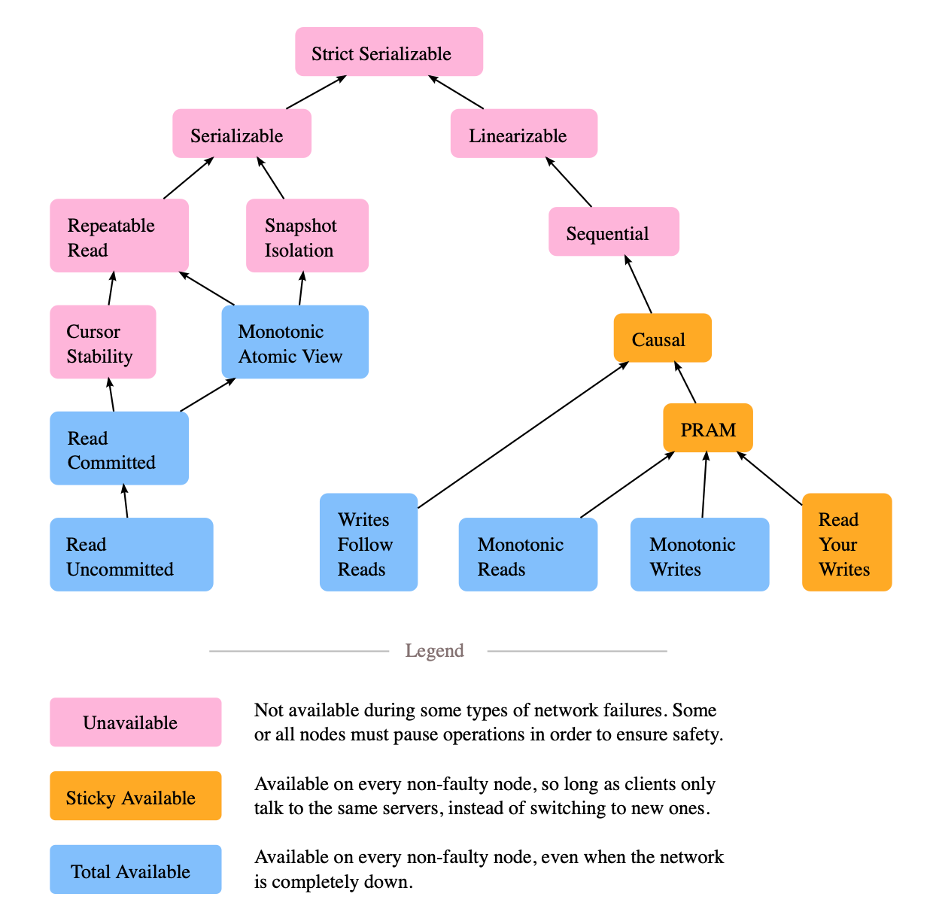
\includegraphics[width=0.85\textwidth]{assets/distributed/jepsen_consistency_models.png}
    \caption{Иерархия моделей согласованности и их доступность}
    \label{fig:jepsen-consistency-tree}
\end{figure}

\textbf{Цветовая схема:}

\begin{itemize}
    \item \textbf{Розовый} — Неустойчива к сбоям сети (unavailable): возможна остановка или невозможность выполнения запросов в ряде сценариев (например, разделённая сеть).
    \item \textbf{Оранжевый} — Липкая доступность (sticky available): работает на каждом неисправном узле, если клиент всегда обращается к одному и тому же серверу, а не переключается на новый. 
    \item \textbf{Голубой} — Полная доступность (total available): работает на каждом неисправном узле, даже если сеть разделена или часть серверов не отвечает.
\end{itemize}

\subsubsection{Обзор основных моделей и их свойств}

\textbf{Strict Serializability (Строгая сериализуемость)}~\\

\textbf{Гарантии:}  ~\\
Результат выполнения нескольких параллельных транзакций такой же, как если бы они выполнялись последовательно.

\textbf{Доступность:}  ~\\
Модель \textit{не достижима} (unavailable) при некоторых типах сбоев: если сеть разделяется или лидер становится недоступен, обработка запросов должна быть остановлена.  

\textbf{Аномалии:}  ~\\
Полное отсутствие аномалий — клиент всегда получает согласованное состояние.\autocite{jepsen-strong-serializable} ~\\

\textbf{Serializable (Сериализуемость)}~\\

\textbf{Гарантии:} ~\\ 
Транзакции в системе выглядят так, будто они были выполнены последовательно, но сериализуемость не требует, чтобы результат чтения всегда отражал последние изменения других клиентов или самого себя из других транзакций. 

\textbf{Доступность:}  ~\\
Аналогично Strict Serializability: unavailable — не поддерживается ни при каких сетевых разрывах.  

\textbf{Аномалии:}  ~\\
Отсутствуют.\autocite{jepsen-serializable}~\\

\textbf{Linearizability (Линеаризуемость)}~\\

\textbf{Гарантии:}  ~\\
Модель согласованности для отдельного объекта, требующая чтобы все транзакции выглядели так, как будто они происходят атомарно в некотором порядке, который согласуется с реальным временем их вызова.

\textbf{Доступность:}  ~\\
Недостижимо при разделении сети (unavailable).  

\textbf{Аномалии:}  ~\\
Отсутствуют.\autocite{jepsen-linearizable}~\\

\textbf{Sequential Consistency (Последовательная согласованность)}~\\

\textbf{Гарантии:}  ~\\
Поддерживает общий последовательный порядок транзакций для всех клиентов. В отличие от линеаризуемости, последовательная согласованность не требует, чтобы этот общий порядок был связан
 с реальным временем исполнения операций. То есть операция B может быть "логически" раньше A даже если в реальности была вызвана позже A.

 \textbf{Доступность:}  ~\\
Недостижимо при разделении сети (unavailable).  

\textbf{Аномалии:}  ~\\
Stale Read: результат чтения может не содержать самых последних записей других процессов, даже если эти записи уже завершены.\autocite{jepsen-sequential}~\\

\textbf{Snapshot Isolation}~\\

\textbf{Гарантии:}  ~\\
Каждая транзакция работает как будто с независимым неизменяемым снимком базы на момент своего старта. Все её изменения видны только ей (до commit). 
После commit они становятся видимы всем, кто начинает транзакцию позже.
Если транзакция пытается изменить объект, который был изменён и зафиксирован другой транзакцией с момента её старта, то будет прервана.

\textbf{Доступность:}  ~\\
Недостижимо при разделении сети (unavailable).  

\textbf{Аномалии:}  ~\\
Возможен write skew: две параллельные транзакции могут прочитать пересекающиеся данные, изменить не пересекающиеся поля и успешно зафиксироваться, вместе нарушая ограничения (например, ограничение суммы).\autocite{jepsen-snapshot-isolation}~\\

\textbf{Repeatable Read}~\\

\textbf{Гарантии:}  ~\\
Читающая транзакция «не видит» изменения данных, которые были ею ранее прочитаны. При этом никакая другая транзакция не может изменять данные, читаемые текущей транзакцией, пока та не окончена.
Однако другие транзакции могут вставлять новые строки, соответствующие условиям поиска инструкций, содержащихся в текущей транзакции. При повторном запуске инструкции текущей транзакцией будут 
извлечены новые строки, что приведёт к фантомному чтению.  

\textbf{Доступность:}  ~\\
Недостижимо при разделении сети (unavailable).  

\textbf{Аномалии:}  ~\\
Возможны фантомные чтения: изменяется результат предикатного запроса за счёт добавления/удаления строк.\autocite{jepsen-repeatable-read}~\\

\textbf{Cursor Stability}~\\ 

\textbf{Гарантии:}  ~\\
Введение понятия "курсора". Курсор указывает на объект, который обрабатывается транзакцией; этот объект нельзя изменять другими транзакциями, 
пока курсор не будет отпущен или пока транзакция не завершится.

\textbf{Доступность:}  ~\\
Недостижимо при разделении сети (unavailable).  

\textbf{Аномалии:}  ~\\
Non-repeatable Read: читая объект вне курсора, можно столкнуться с тем, что значение этого объекта изменится другой транзакцией в ходе одной и той же транзакции (неповторяемое чтение) 
и Phantom: набор строк по предикату может измениться.\autocite{jepsen-cursor-stability}~\\

\textbf{Monotonic Atomic View}~\\

\textbf{Гарантии:}  ~\\
Любая транзакция либо видит полные результаты (все изменения) другой транзакции, либо не видит ничего из них.
Предотвращается ситуация, когда часть изменений уже видна, а часть — ещё нет.

\textbf{Доступность:}  ~\\
Полностью доступна (total available) — даже при разделениях сети каждый узел может продолжать работать.

\textbf{Аномалии:}  ~\\
Non-repeatable Read и Phantom \autocite{jepsen-monotonic-atomic-view}~\\

\textbf{Read Committed}~\\

\textbf{Гарантии:}  ~\\
Модель согласованности, усиливающая read uncommitted тем, что не позволяет чтение незафиксированных данных (dirty reads): транзакция не может видеть изменения, 
сделанные другой транзакцией, пока та не выполнит commit.

\textbf{Доступность:}  ~\\
Полностью доступна (total available) — даже при разделениях сети каждый узел может продолжать работать.

\textbf{Аномалии:}  ~\\
Non-repeatable read, phantom read.\autocite{jepsen-read-committed}~\\

\textbf{Read Uncommitted}~\\

\textbf{Гарантии:}  ~\\
Читаются любые значения, даже незафиксированные. Она обеспечивает только то, что не будет “грязных записей” (dirty write):  
когда две транзакции одновременно изменяют один и тот же объект перед фиксацией.

\textbf{Доступность:}  ~\\
Полностью доступна (total available) — даже при разделениях сети каждый узел может продолжать работать.

\textbf{Аномалии:}  ~\\
Запрещено только Dirty Write: не допускаются ситуации, когда две транзакции одновременно модифицируют одну запись\autocite{jepsen-read-uncommitted}~\\

\textbf{Causal Consistency}~\\

\textbf{Гарантии:}  ~\\
Все операции, связанные причинно-следственно (“happens-before”), будут наблюдаться всеми процессами в одном и том же порядке, 
хотя порядок независимых операций может различаться для разных клиентов.

\textbf{Доступность:}  ~\\
Sticky Available — клиенты должны придерживаться одного и того же сервера.

\textbf{Аномалии:}  ~\\
Если две транзакции или действия причинно не связаны, то разные клиенты могут видеть их в разном порядке.\autocite{jepsen-causal}~\\

\textbf{Writes Follow Reads}~\\

Если процесс прочитал некоторое значение $v$, возникшее после записи $w_1$, а затем сам выполняет запись $w_2$, то для всех остальных процессов $w_2$ станет видимой только после того, как станет видимым $w_1$.  
Иными словами, запись не может «переписать прошлое» тех данных, которые уже были прочитаны.\autocite{jepsen-writes-follow-reads}~\\

\textbf{PRAM (Pipeline Random Access Memory)}~\\

Все операции (записи), выполненные одним процессом, всегда наблюдаются всеми остальными процессами в том же порядке, в каком были исполнены этим процессом. Однако записи разных процессов могут быть видны на других узлах в разном порядке.\autocite{jepsen-pram}~\\


\textbf{Monotonic Reads}~\\

Если процесс последовательно выполняет чтения $r_1$, затем $r_2$, то $r_2$ никогда не увидит состояние системы, "старее" тех изменений, что были видны при $r_1$.  
То есть, чтения не могут “откатиться назад”: процесс не увидит более старое состояние после того, как уже увидел более новое. \autocite{jepsen-monotonic-reads}~\\


\textbf{Monotonic Writes}~\\

Если процесс выполняет сначала запись $w_1$, затем запись $w_2$, то все другие процессы никогда не увидят $w_2$ без того, чтобы не увидеть $w_1$ раньше.  
То есть, серию записей одного процесса другие клиенты всегда наблюдают в том же порядке, что и процесс их выполнил.\autocite{jepsen-monotonic-writes}~\\

\textbf{Read Your Writes}~\\

Если процесс совершает запись $w$, а затем выполняет чтение $r$, то $r$ обязательно увидит результат $w$ (то есть, то, что только что было записано этим же процессом).
Нет никаких гарантий для других процессов: если клиент 1 записал значение, клиент 2 не обязан увидеть это значение сразу же.\autocite{jepsen-read-your-writes}~\\


